\documentclass[12pt]{article}

% ─── Packages ─────────────────────────────────────────────────────────────────
\usepackage[a4paper, margin=2.54cm, headheight=14pt]{geometry}
\usepackage{setspace}
\usepackage{times}
\usepackage{amsmath, amssymb}
\usepackage{booktabs}
\usepackage{array}
\usepackage{graphicx}
\usepackage{hyperref}
\usepackage[authoryear,round,sort]{natbib}
\setlength{\bibsep}{2pt}
\usepackage{fancyhdr}
\usepackage{titlesec}
\usepackage{microtype}
\usepackage[T1]{fontenc}
\usepackage[utf8]{inputenc}
\usepackage{caption}
\usepackage{float}
\usepackage[section]{placeins}
\usepackage{algorithm}
\usepackage{algpseudocode}

% ─── Spacing & Layout ─────────────────────────────────────────────────────────
\doublespacing
\setlength{\parindent}{0.5in}
\setlength{\parskip}{0pt}

% ─── Header / Footer ──────────────────────────────────────────────────────────
\pagestyle{fancy}
\fancyhf{}
\rhead{\small\MakeUppercase{Null models for rule-defined pattern counts}}
\rfoot{\thepage}
\renewcommand{\headrulewidth}{0pt}

% ─── Section formatting ───────────────────────────────────────────────────────
\titleformat{\section}{\normalfont\normalsize\bfseries}{\thesection.}{0.5em}{}
\titleformat{\subsection}{\normalfont\normalsize\bfseries}{\thesubsection}{0.5em}{}
\titleformat{\paragraph}[runin]{\normalfont\normalsize\bfseries}{}{0pt}{}[\ ---]
\titlespacing*{\section}{0pt}{12pt}{6pt}
\titlespacing*{\subsection}{0pt}{10pt}{4pt}
\titlespacing*{\paragraph}{0pt}{6pt}{0.5em}

\hypersetup{colorlinks=true, linkcolor=blue, citecolor=blue, urlcolor=blue,
  pdftitle={Null-Model Choice for Rule-Defined Pattern Counts in Clustered Longitudinal Sequences: A Case Study of Jewish Halachic Menstrual Anticipation Rules},
  pdfauthor={Dvir Ross}}
\newcolumntype{L}[1]{>{\raggedright\arraybackslash}p{#1}}
\newcolumntype{C}[1]{>{\centering\arraybackslash}p{#1}}
\graphicspath{{figures/}}
\captionsetup{font=small, labelfont=bf, width=0.92\textwidth}

\providecommand{\doi}{}
\renewcommand{\doi}[1]{\href{https://doi.org/#1}{\nolinkurl{https://doi.org/#1}}}
\newcommand{\HG}{H_{G}}
\newcommand{\HI}{H_{iid}}
\newcommand{\HW}{H_{W}}
\newcommand{\DM}{D_{M}}

% ══════════════════════════════════════════════════════════════════════════════
\begin{document}

% ─── Title Page ───────────────────────────────────────────────────────────────
\begin{titlepage}
  \centering
  \vspace*{0.4cm}
  {\large\bfseries Null-Model Choice for Rule-Defined Pattern Counts in Clustered
  Longitudinal Sequences:\\[4pt]
  \normalfont\large A Case Study of Jewish Halachic Menstrual Anticipation Rules\par}
  \vspace{0.7cm}
  {Dvir Ross\par}
  \vspace{0.2cm}
  {\small ORCID: \href{https://orcid.org/0000-0001-8217-3359}{0000-0001-8217-3359}\par}
  \vspace{0.4cm}
  \begin{minipage}[t]{0.46\textwidth}
    \centering\small\itshape
    Department of Software Engineering\\
    Shenkar College of Engineering, Design and Art\\
    12 Anne Frank St.\\
    Ramat Gan 5252626, Israel
  \end{minipage}\hfill
  \begin{minipage}[t]{0.46\textwidth}
    \centering\small\itshape
    Department of Computer Science\\
    SCE --- Shamoon College of Engineering\\
    56 Bialik Street, P.O.B.\ 950\\
    Beer Sheva 8410802, Israel
  \end{minipage}
  \vspace{0.6cm}
  \begin{spacing}{1.0}
  {\normalsize\bfseries Author Note\par}
  \vspace{0.2cm}
  \begin{flushleft}
  Article type: Case Study.

  \medskip
  The dataset analysed in this study is the publicly archived Marquette University
  menstrual cycle dataset \citep{fehring2012data}, collected in the randomised trial of
  \citet{fehring2013}. The author declares no conflicts of interest. Analysis code, the
  filtered dataset and cached Monte Carlo replicates are available at
  \url{https://github.com/dvirross/VessetVectorTest}.

  \medskip
  \textbf{Correspondence:} Dvir Ross, Department of Software Engineering, Shenkar
  College of Engineering, Design and Art, 12 Anne Frank St., Ramat Gan 5252626, Israel.
  Email: \texttt{dvirross@shenkar.ac.il} (additional: \texttt{RossDv@sce.ac.il}).
  \end{flushleft}
  \vspace{0.4cm}
  {\normalsize\bfseries Acknowledgments\par}
  \vspace{0.2cm}
  \begin{flushleft}\small
During manuscript preparation in 2026, the author used ChatGPT (OpenAI, GPT-5.6 Sol),
  Gemini (Google, Deep Research using Gemini 3.1 Pro), Perplexity (Deep Thinking mode; the
  underlying model was not identified by the interface), and Claude/Claude Code (Anthropic,
  using Claude Sonnet 4.6 and Claude Fable 5.1). ChatGPT, Gemini and Perplexity were used
  for critical review, research support, editorial feedback and manuscript preparation.
  Claude/Claude Code was used for critical review and manuscript editing, and also to
  generate or refactor portions of the Python and \LaTeX{} code. All AI-assisted
  suggestions and code were reviewed, tested and revised by the author. All scientific
  content, analytical decisions, interpretations and conclusions are the author's, who
  takes full responsibility for the accuracy and integrity of the article.
  
    This research received no specific grant from any funding agency in the public,
  commercial, or not-for-profit sectors.
  \end{flushleft}
  \end{spacing}
\end{titlepage}

% ─── Abstract ─────────────────────────────────────────────────────────────────
\newpage
\begin{center}{\bfseries Abstract}\end{center}

\noindent
The evidential weight of counts of deterministically defined patterns in clustered
longitudinal sequences can depend strongly on the exchangeability null used to define
``chance'': the same excess
can be generated by heterogeneity between subjects or by ordering within subjects, and
the counts are typically small, integer-valued and dependent by construction. We
illustrate the problem with menstrual-cycle patterns defined by Jewish religious law
(\textit{Halacha}), whose \textit{vesset} rules require a woman to anticipate
menstruation from exact arithmetic events in her history of inter-menstrual intervals ---
three equal consecutive intervals, a constant first or second difference, a repeated
weekly anchor. We analyse 1,554 cycles from 118 women under three exchangeability nulls
for the same five-count vector: a global permutation null, a multinomial i.i.d.\ null,
and a within-woman permutation null that conditions on each woman's multiset of cycle
lengths and randomises only their order. All are evaluated with two-sided Monte Carlo
marginal tests and a joint quadratic-form (Mahalanobis) permutation statistic whose
covariance is estimated from the null replicates. Under the global nulls the count
vector is displaced far into the tail ($\DM = 5.08$, $p < .001$; Haflaga $z = 4.50$).
Under the within-woman null it is not ($\DM = 2.93$, $p = .13$; smallest Holm-adjusted
marginal $p = .19$), and all five observed counts lie at or below their conditional null
means. Simulation shows type-I error at or below the nominal level for the marginal and
Holm procedures and approximately nominal for the joint test, quantifies the power of
the within-woman tests against simulated autoregressive and exact-repetition
alternatives, and shows the conclusions are insensitive to unequal follow-up. The
contrast is consistent with between-woman heterogeneity in regularity generating the
global excess, and provides no evidence that within-woman ordering produces additional
rule-defined events; it does not establish the absence of serial dependence.

\medskip
\noindent\textit{Keywords:} exchangeability, Halacha, menstrual cycle, permutation test,
within-subject null

% ─── 1. Introduction ──────────────────────────────────────────────────────────
\newpage
\section{Introduction}

Menstrual cycle length varies both within and between women
\citep{munster1992,creinin2004,harlow2000,bull2019}. The population distribution is
bell-shaped with a pronounced right tail; within-woman consistency is moderate, with
intraclass correlations typically between $0.3$ and $0.5$ \citep{dasharathy2012}, and
the menstrual cycle is increasingly treated as a within-person process requiring
within-person modelling \citep{schmalenberger2021}. Hierarchical state-space models
exploit this structure for cycle-length prediction \citep{bortot2010}, and recent
multi-cohort work documents low-order autocorrelation in cycle lengths
\citep{ecochard2024}.

In Jewish religious law (\textit{Halacha}) this regularity is also the object of a
detailed legal system. A woman is required to anticipate the onset of her next
menstruation from patterns in her prior cycle history; the anticipatory rules --- the
\textit{halachic vesset rules} (\textit{vesset}: menstruation) --- govern abstinence
obligations within \textit{taharat hamishpacha}, the laws of family purity. Each rule
defines an exact arithmetic event in the sequence of inter-menstrual intervals. Of the 17
rule types in the halachic literature, 10 require calendar or time-of-day data that
standard cycle records do not contain; 7 are computable from interval lengths alone.
Despite centuries of practical application and the availability of longitudinal cycle
datasets, we are not aware of any formal randomisation-based test of whether the
frequency of these events in empirical data departs from what chance would produce (no
systematic literature search was performed).

From a statistical point of view the question is a case of a general problem: testing
whether counts of deterministically defined patterns in clustered longitudinal sequences
depart from a null expectation, when (i) subjects contribute sequences of very unequal length
(here 5--45 cycles), (ii) the counts are integer-valued and small, (iii) the counts are
dependent by definition (one rule's event set is a subset of another's), and (iv) the
same excess can be generated either by heterogeneity between subjects or by ordering
within subjects. The choice of null is therefore not a technicality. Randomisation tests
derive their validity from the exchangeability structure they impose
\citep{edgington2007,good2005}; permutation inference for longitudinal and clustered
data has been studied extensively \citep{friedrich2017,lee2012}, exchangeability-block
permutation is standard in
neuroimaging \citep{nichols2002,winkler2014}, and conditional permutation tests that
hold part of the data structure fixed have a modern theory
\citep{berrett2020,hemerik2018}. This paper applies these established tools to the
vesset counts and uses the application to make one point concrete: for the same data,
a population-level exchangeability null and a within-subject conditional null return
diametrically different answers, and only the latter addresses the question the rules
implicitly pose.

We compare three nulls --- a global permutation null $\HG$, a multinomial i.i.d.\ null
$\HI$ and a within-woman permutation null $\HW$ --- using the same two-sided Monte Carlo
marginal tests and the same joint quadratic-form statistic, a Mahalanobis distance from
the simulated null mean with covariance estimated from the null replicates. The joint
statistic is an adaptation of well-known quadratic-form permutation tests
\citep{anderson2001,pesarin2010,szekely2013}; we make no claim of methodological
novelty for it and instead verify its calibration by simulation. The study extends a
line of quantitative halachic scholarship \citep{ross2022markov,ross2019reliability,
ross2021statistical,ross2022phd} and is presented as a Case Study.

% ─── 2. Background ────────────────────────────────────────────────────────────
\section{Background}

\subsection{The Polynomial Hierarchy of Vesset Rules}

Let $L_1, \ldots, L_n$ denote one woman's cycle lengths (days) and define the
\textit{haflaga} $H_k = L_k + 1$, the interval from the first day of menstruation $k$ to
the first day of menstruation $k+1$, following halachic convention
\citep{ross2021statistical}. The five rule types analysed here are:

\begin{description}
  \item[\textit{Haflaga.}] $H_k = H_{k-1} = H_{k-2}$: three or more consecutive equal
    haflaga values. Degree-0 (constant) sequence; minimum run 3 cycles.
  \item[\textit{Dilug.}] $H_k - H_{k-1} = H_{k-1} - H_{k-2} = d \neq 0$: constant
    non-zero first difference. Degree-1 (linear); minimum run 3.
  \item[\textit{Dilug-in-Dilug.}] Constant non-zero second difference,
    $(H_k - H_{k-1}) - (H_{k-1} - H_{k-2}) = (H_{k-1} - H_{k-2}) - (H_{k-2} - H_{k-3})
    = d \neq 0$. Degree-2 (quadratic); minimum run 4.
  \item[\textit{Week.}] $H_k = H_{k-1} \in \mathcal{W}$, where
    $\mathcal{W} = \{H_{\min}+3, H_{\min}+10, \ldots\}$ are values spaced 7 apart
    (same weekday at each onset). Degree-0 anchored to weekly values; minimum run 2.
  \item[\textit{Week-Dilug.}] $H_k = H_{k-1} = 30$. A haflaga of 30 (29 days, four weeks
    plus one day) is the unique interval for which each successive onset falls one
    weekday later, producing an arithmetic progression of weekdays --- hence the name
    (Hebrew \textit{shavu'a be-dilug}; \citealp{ross2022phd}). Degree-0 at the canonical
    anchor; minimum run 2.
\end{description}

Haflaga, Dilug and Dilug-in-Dilug follow increasing polynomial order in cycle index;
Week and Week-Dilug are specialisations of the degree-0 case anchored to calendar
values. Two further computable rules (\textit{Dilug Chozer Chalila} and \textit{Haflaga
Chozer Chalila}, repeating multi-value cycles of intervals) require windows of at least
six to nine cycles; they are discussed in Section~\ref{sec:data}.

\subsection{Dependence Structure Implied by the Definitions}
\label{sec:mathdep}

Two relationships follow from the definitions and are relevant to how the counts should
be tested jointly.

\paragraph{Haflaga-30 $\subseteq$ Week-Dilug (deterministic containment).}
Week-Dilug requires two consecutive haflaga values equal to 30; a Haflaga sequence with
value 30 requires three. Every Haflaga-30 sequence therefore generates a Week-Dilug
event in its first two cycles. This is set-theoretic inclusion, not a stochastic
association: in the data, the 3 Haflaga sequences with $H = 30$ contribute directly to
the Week-Dilug count of 18.

\paragraph{Haflaga and Dilug-in-Dilug (algebraic proximity).}
When the second difference $|d|$ of a Dilug-in-Dilug sequence is 1, its first
differences change by one day per cycle and the haflaga sequence is nearly constant. In
the data, 16 of 27 Dilug-in-Dilug sequences have $|d| = 1$. This makes positive
co-occurrence with Haflaga plausible but does not entail it.

A third relation, mutual exclusion of Dilug ($\Delta H \neq 0$) and Week-Dilug
($\Delta H = 0$) within the same window, implies a weak negative tendency for that pair.
The five counts are thus non-independent by construction, which motivates estimating
their joint null covariance rather than treating them as separate tests.

\subsection{Prior Work and Dataset Overlap}
\label{sec:prior}

Statistical characterisation of cycle-length variability is extensive
\citep{munster1992,creinin2004,harlow2000,fehring2006,dasharathy2012,symul2019,bull2019},
and hierarchical models for sequential prediction exist \citep{bortot2010}. Quantitative
halachic analyses have modelled cycle transitions with Markov chains
\citep{ross2022markov}, examined the reliability of self-reported cycle data in a
halachic setting \citep{ross2019reliability}, and analysed abstinence rules
statistically; none tested pattern frequencies against a randomisation null.

\citet{ecochard2024} report evidence of an internal circamonthly oscillator using
multi-cohort data that include a North American cohort collected by Fehring and
Schneider, two of the investigators of the trial from which the dataset analysed here
was drawn \citep{fehring2012data,fehring2013}.
Their Marquette cohort (1,649 cycles, 159 women) and the present sample (1,554 cycles,
118 women after exclusions) are probably drawn from the same data-collection
infrastructure and should not be regarded as independent samples. They document second-
to fourth-order autocorrelation in cycle lengths. We note the implication for $\HW$
precisely: within-woman permutation preserves each woman's multiset of cycle lengths
and her sequence length, and \emph{destroys} the observed ordering and therefore any
serial dependence. Autocorrelation is not preserved under $\HW$; rather, $\HW$ is the
reference distribution in which it is absent, so a rejection of $\HW$ would indicate
ordering structure that produces rule-defined events, and a non-rejection indicates only
that these specific count statistics are not unusual relative to random reorderings of
each woman's own values.

% ─── 3. Methods ───────────────────────────────────────────────────────────────
\section{Methods}
\label{sec:methods}

\subsection{Dataset}
\label{sec:data}

We analysed the publicly archived longitudinal dataset of \citet{fehring2012data},
collected in a randomised trial of two Internet-supported fertility-awareness-based
methods of family planning \citep{fehring2013}; we refer to the participants as natural
family planning (NFP) users. The archived file contains 1,665 cycles from 159 women.
Every recorded cycle length in it lies between 18 and 54 days and none is missing, so no
cycle-length criterion was applied by us; whether the archive itself was restricted to
this range by the original investigators is not documented in the materials available
to us. Three women whose cycle records appeared twice in the archive (16 rows in total,
each with at most three distinct cycles) were removed, women with fewer than 5 recorded
cycles were excluded (38 women, 87 cycles), and for one further woman whose eight cycles
appeared as two near-identical copies (differing in one recorded length) a single copy
was retained. The analysed sample comprises
\textbf{1,554 cycles from 118 women} ($M = 13.2$ cycles per woman, SD $= 6.1$, range
5--45). Cycle lengths ranged from 18 to 54 days ($M = 29.3$, SD $= 3.9$, Mdn $= 28.5$,
skewness $= 1.29$); 9.6\% of cycles were 35 days or longer. The source trial
(ClinicalTrials.gov NCT00843336) enrolled women aged 18--42 years who reported cycle
lengths of 21--42 days at entry \citep{fehring2013}; in the analysed sample age is recorded for
99 of the 118 women and ranges from 21 to 43 years ($M = 31.8$, SD $= 5.4$). Parity was
not recorded. The data come from two charting
cohorts ($n = 69$ and $49$ women in the filtered sample); cohort membership was not used
in the analysis. All lengths were incremented by 1 to the haflaga convention, giving
$M = 30.3$, SD $= 3.9$.

Because the pattern detectors operate on \emph{consecutive} cycles, it matters whether
the exclusions could have created artificial adjacency across a removed cycle. They
could not: the filtering removed whole women or duplicated rows only, and in the filtered
file every woman's recorded \texttt{CycleNumber} runs $1, 2, \ldots, n_i$ without gaps
(verified programmatically and asserted in the analysis code), so no pattern window spans
an excluded cycle. The five-cycle minimum ensures that every retained woman can in
principle produce each of the five pattern types, the longest of which requires four
consecutive intervals. The filtering script is part of the code release and reproduces
the filtered file exactly from the archived source file (Section~\ref{sec:das}).

Of the seven rule types computable from cycle-length data, the two repeating-cycle rules
(\textit{Dilug Chozer Chalila}, \textit{Haflaga Chozer Chalila}) had no observed
occurrences. The five-pattern family analysed here was therefore selected after
inspection of the observed data and should be regarded as data-informed rather than
pre-specified; the two zero-occurrence rules were not implemented in the analysis code
and were not included in the multivariate analysis or in the Holm family. The analyses
reported below are accordingly described as primary rather than confirmatory.

As a descriptive characterisation, the 20 women with at least one Haflaga event had a
mean within-woman SD of cycle length of 1.54 days (between-woman SD 0.59), compared with
3.17 days (1.75) for the 35 women with no event of any type (Mann--Whitney $U = 133$,
$p < .001$; Welch $t = -5.05$, df $= 45.5$; 95\% CI for the difference
$[-2.29, -0.98]$ days; Cohen's $d = -1.13$). Because Haflaga is \emph{defined} by
repeated equal intervals, a lower SD among these women is expected by construction; this
comparison describes the women the rule selects and is not independent validation of the
rule. Within-woman SD estimates also depend on the number of cycles observed (5--45).
Figure~\ref{fig:dist} shows the distribution and per-woman variability;
Figure~\ref{fig:consort} summarises the data flow.

\begin{figure}[!htbp]
  \centering
  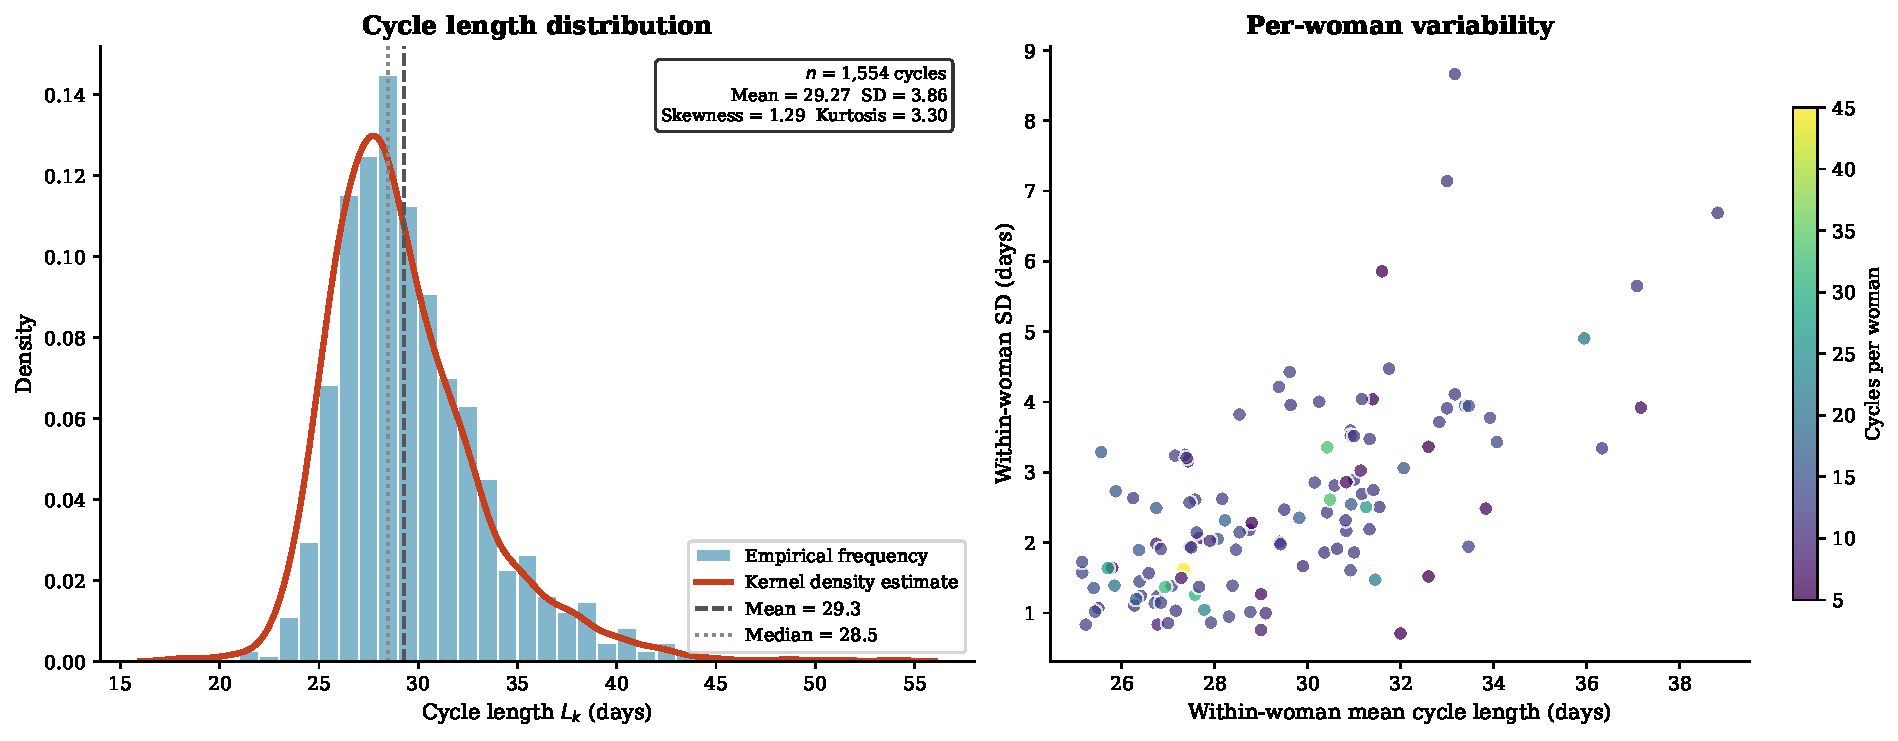
\includegraphics[width=\textwidth]{fig1_cycle_distribution}
  \caption{Cycle length distribution (filtered dataset). \textit{Left}: histogram and
    kernel density estimate of $L_k$ with mean (dashed) and median (dotted); skewness
    $= 1.29$. \textit{Right}: per-woman mean vs.\ within-woman SD, shaded by cycle count.}
  \label{fig:dist}
\end{figure}

\begin{figure}[!htbp]
  \centering
  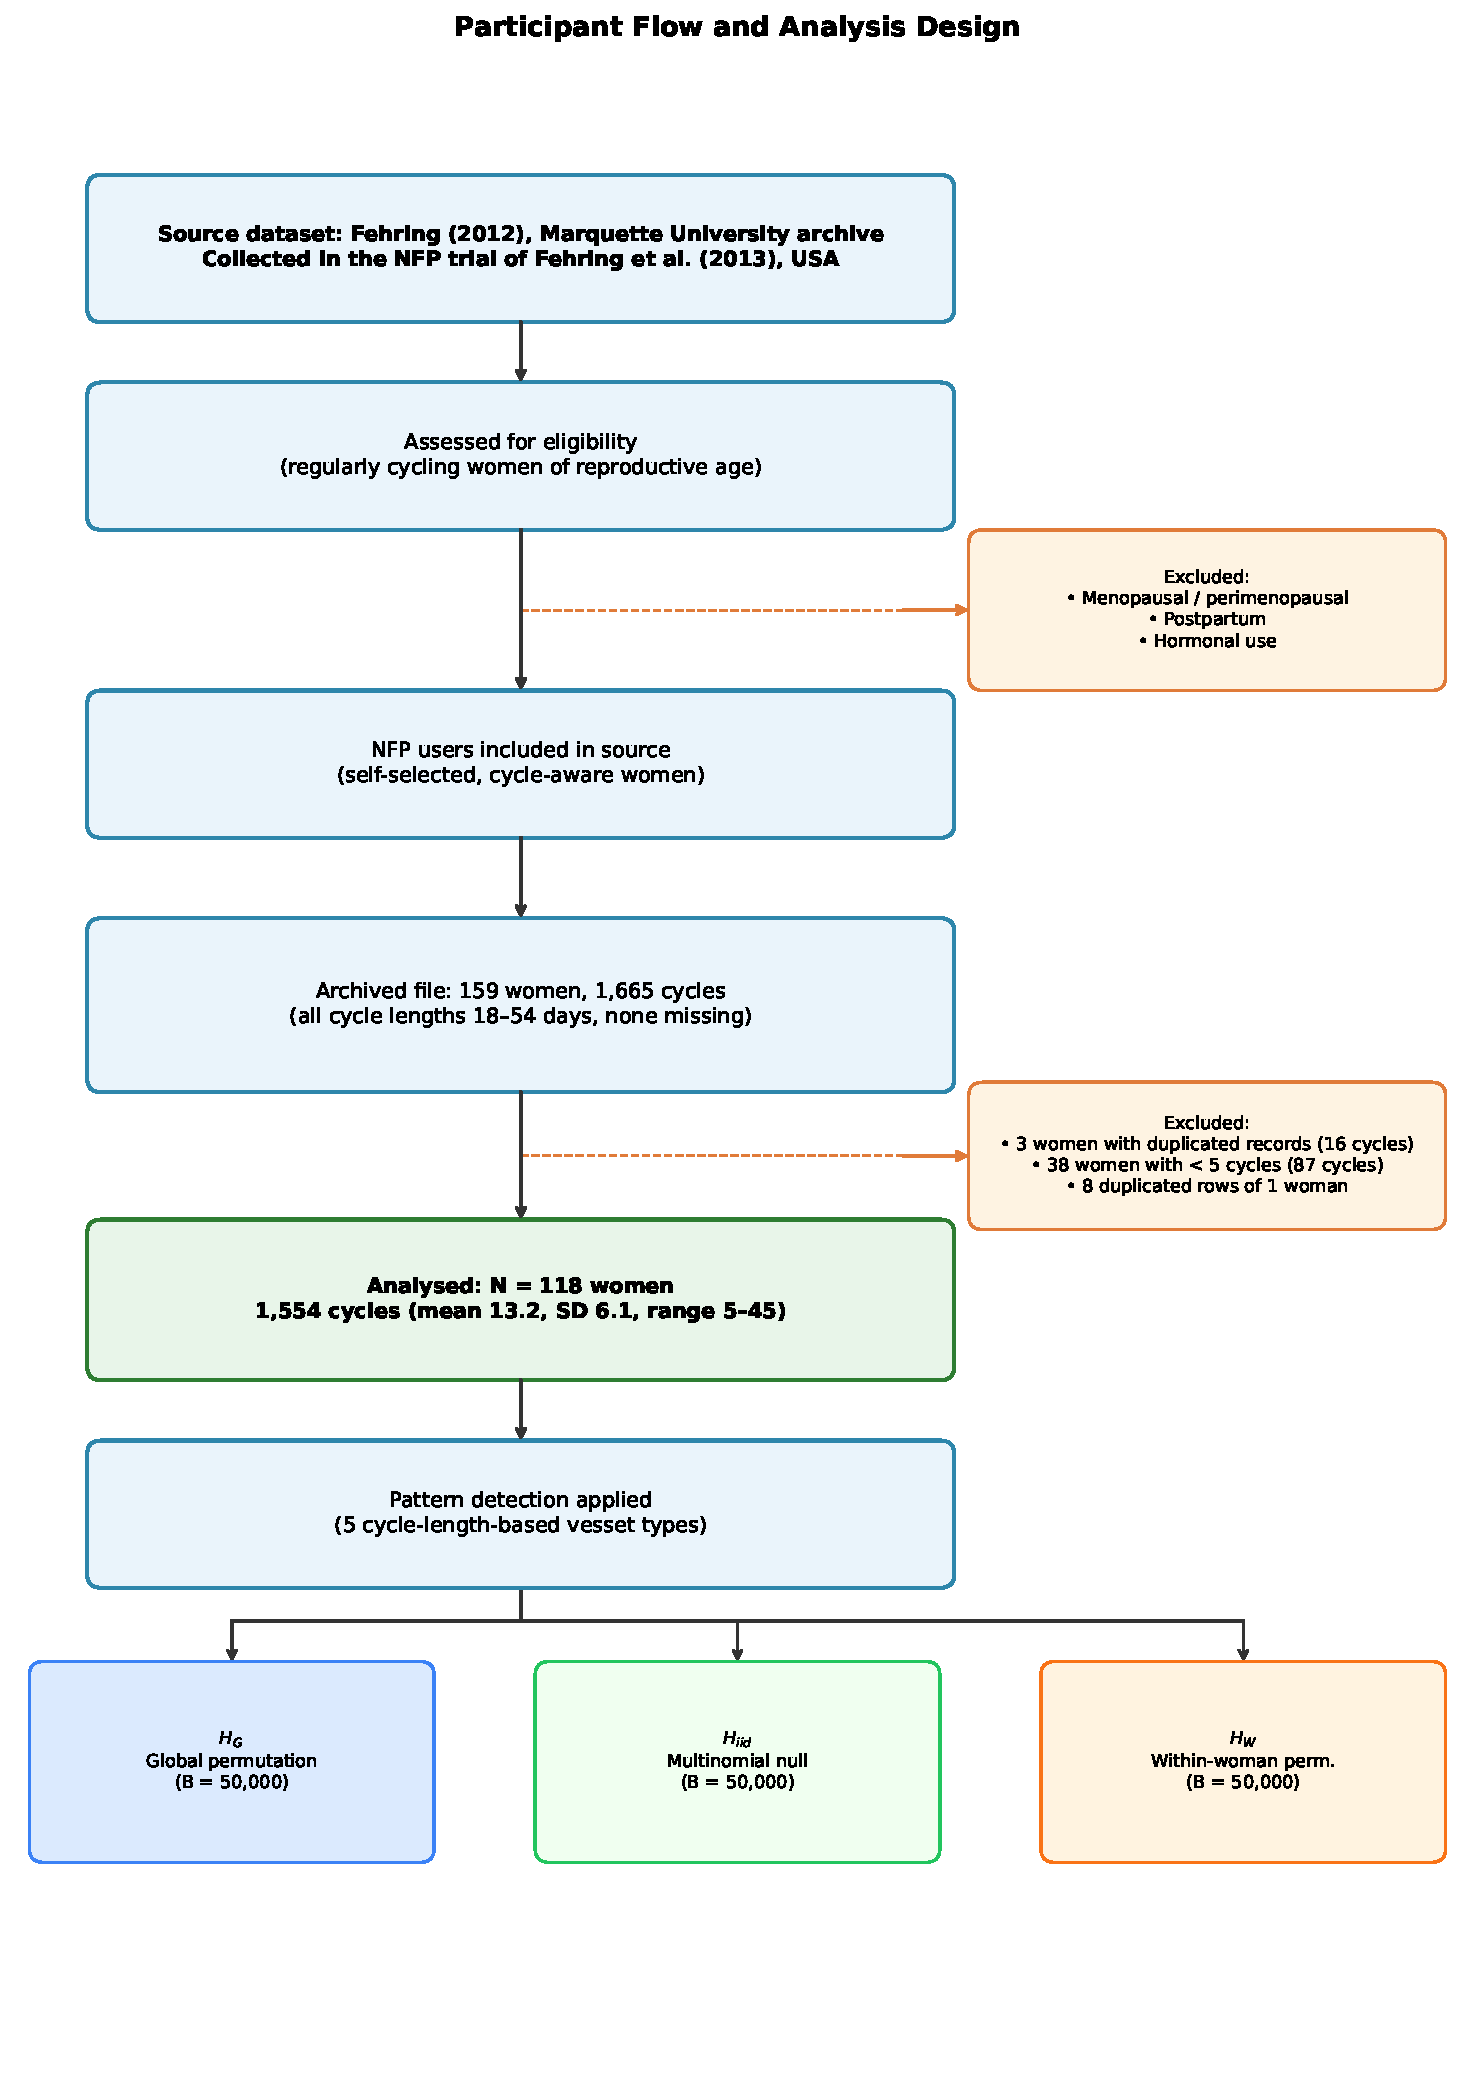
\includegraphics[width=0.75\textwidth]{fig2_consort_flow}
  \caption{Participant and data flow. Source dataset \citep{fehring2012data}, collected
    in the trial of \citet{fehring2013}; archived file of 159 women and 1,665 cycles;
    exclusion of women with duplicated cycle records or fewer than 5 cycles; analysed
    sample of 118 women and 1,554 cycles; five pattern types; three null models, each with
    $B = 50{,}000$ replicates.}
  \label{fig:consort}
\end{figure}

\subsection{Pattern Detection}
\label{sec:detect}

Counting is performed within each woman's sequence; sequences are never concatenated
across women, and the woman boundaries $(s_i, f_i)$ are enforced in every counting loop.
Each function counts \emph{distinct maximal contiguous runs} satisfying its rule: a run
longer than the minimum counts once (four equal haflaga values are one Haflaga event), and
a qualifying run that resumes after a discordant cycle counts again. To fix the
convention: $(29, 29)$ qualifies as Week (if $29 \in \mathcal{W}$) but not as Haflaga;
$(28, 28, 28)$ is a Haflaga; $(27, 29, 31, 33)$ is a Dilug ($d = 2$) with second
differences $(0, 0)$ and hence not a Dilug-in-Dilug; $(27, 28, 30, 33)$ has first
differences $(1, 2, 3)$ and second differences $(1, 1)$ and is a Dilug-in-Dilug.

Two implementations were written --- a reference loop version and a vectorised version
used for simulation --- and checked to agree on the observed data and on 9,000 random
null sequences. Portions of the analysis code were generated or refactored with
assistance from Claude/Claude Code (Anthropic; Claude Sonnet 4.6 and Claude Fable 5.1);
all AI-assisted code was reviewed and tested by the author, and the pattern-counting code
is additionally checked by this two-implementation equivalence test. The observed count
vector is
$\mathbf{O} = (26, 61, 32, 18, 27)$ for (Haflaga, Dilug, Week, Week-Dilug,
Dilug-in-Dilug). The code, the filtered data, and all Monte Carlo replicates are
available at \url{https://github.com/dvirross/VessetVectorTest}.

\subsection{Null Models}
\label{sec:nullmodels}

Three nulls encode three scientific questions (Table~\ref{tab:nullmodels}).
\begin{description}
  \item[$\HG$ \textnormal{(global).}] All 1,554 haflaga values are
    exchangeable across women: the pooled values are permuted without replacement and
    re-assigned to women preserving each $n_i$. Tests whether the counts exceed what a
    homogeneous population would produce.
  \item[$\HI$ \textnormal{(multinomial).}] Each woman's $n_i$ values are drawn
    independently from the pooled empirical distribution $\hat F$ \citep{ross2022phd}.
    Stronger than $\HG$ in that observed values, not only their ordering, are replaced.
  \item[$\HW$ \textnormal{(within-woman).}] Conditional on each woman's
    observed multiset $\{H_{i,1}, \ldots, H_{i,n_i}\}$ and on $n_i$, all $n_i!$ orderings
    are equally likely. Each woman's sequence is permuted uniformly at random without
    replacement (indices are permuted, so ties are handled exactly). This is a
    conditional Monte Carlo test \citep{hemerik2018}: it preserves each woman's level of
    regularity and cycle count, destroys within-woman ordering, and tests whether the
    ordering generates rule-defined events beyond what her own values in random order
    would. It is not a general test of serial independence: an autocorrelated or trending
    process that does not produce additional exact events will not reject it.
\end{description}

\begin{table}[!htbp]
\centering
\caption{The three null models.}
\label{tab:nullmodels}
\small
\begin{tabular}{L{3.0cm} L{3.7cm} L{3.7cm} L{3.7cm}}
\toprule
& $\HG$ (global permutation) & $\HI$ (multinomial) & $\HW$ (within-woman permutation) \\
\midrule
\textbf{Randomised} & assignment of pooled cycle values to positions & each value, drawn i.i.d.\ from $\hat F$ & order of each woman's own values \\[3pt]
\textbf{Preserved} & pooled multiset; each $n_i$ & each $n_i$; pooled proportions & each woman's multiset and $n_i$ \\[3pt]
\textbf{Destroyed} & woman identity; ordering & all dependence; heterogeneity & within-woman ordering only \\[3pt]
\textbf{Scientific null} & counts arise from a homogeneous population & counts arise from independent draws & counts arise from random ordering of each woman's values \\
\bottomrule
\end{tabular}
\end{table}

A within-woman \emph{bootstrap} (sampling each woman's values with replacement) was
considered and rejected as the conditional null: with-replacement draws are independent,
whereas permutation draws are negatively dependent (a value used at one position is less
available at the next), so the bootstrap inflates the expected count of repetition-based
patterns (Haflaga null mean 54.5 vs.\ 31.8; verified with $B = 50{,}000$). The two
procedures encode different nulls --- i.i.d.\ resampling versus exchangeability of the
observed values --- and are not more or less conservative versions of one another;
permutation is the exact conditional test for the stated exchangeability null.

\subsection{Statistical Inference}
\label{sec:inference}

For pattern $j$ and null $m$, with $B = 50{,}000$ replicate count vectors
$\mathbf{S}^{(m,r)}$, we report the null mean $\bar S_j^{(m)}$ and SD $\sigma_j^{(m)}$,
the standardised departure $z_j^{(m)} = (O_j - \bar S_j^{(m)})/\sigma_j^{(m)}$, and the
two-sided Monte Carlo $p$-value
\begin{equation}
  p_j^{(m)} = \min\Bigl\{1,\; 2\min\Bigl(\tfrac{b_j^+ + 1}{B+1},\, \tfrac{b_j^- + 1}{B+1}\Bigr)\Bigr\},
  \label{eq:ptwo}
\end{equation}
where $b_j^+ = \#\{r : S_j^{(m,r)} \geq O_j\}$ and $b_j^- = \#\{r : S_j^{(m,r)} \leq O_j\}$,
following the $(b+1)/(B+1)$ convention \citep{davison1997,phipson2010}. The same
convention is used everywhere (tables, figures, algorithm). Two-sided tests are used
because departures in either direction are informative for these rules. Across the five
marginal tests the family-wise error rate is controlled by Holm's step-down procedure,
which is valid under arbitrary dependence.

The \textbf{joint test} uses the Mahalanobis distance of $\mathbf{O}$ from the simulated
null mean,
\begin{equation}
  \DM^{(m)} = \sqrt{\bigl(\mathbf{O}-\hat{\boldsymbol{\mu}}^{(m)}\bigr)^\top
               \bigl(\hat{\Sigma}^{(m)}\bigr)^{-1}
               \bigl(\mathbf{O}-\hat{\boldsymbol{\mu}}^{(m)}\bigr)},
  \label{eq:mahalanobis}
\end{equation}
where $\hat{\boldsymbol{\mu}}^{(m)}$ and $\hat\Sigma^{(m)} = (B-1)^{-1}\sum_r
(\mathbf{S}^{(m,r)} - \bar{\mathbf{S}}^{(m)})(\mathbf{S}^{(m,r)} - \bar{\mathbf{S}}^{(m)})^\top$
are the mean and sample covariance of the null replicates (not of the observations).
The $p$-value is the fraction of replicates whose own $\DM$, computed with the same
$\hat{\boldsymbol{\mu}}$ and $\hat\Sigma$, is at least the observed value, again with the
$(b+1)/(B+1)$ convention. This is a single global test of the multivariate null and is
inherently two-sided; it is a standard permutation quadratic form
\citep{anderson2001,pesarin2010} closely related to Hotelling's $T^2$ with the
parametric reference distribution replaced by a Monte Carlo one, and to energy-distance
tests \citep{szekely2013}. Because the same replicates estimate $\hat\Sigma$ and form the
reference distribution, we also report a \textbf{split-batch} version
($\hat{\boldsymbol{\mu}}, \hat\Sigma$ from the first 25,000 replicates; reference
distribution from the last 25,000) and verify calibration by simulation
(Section~\ref{sec:simdesign}). Condition numbers of $\hat\Sigma$ (4.4--5.4) indicate a
numerically stable inversion; they say nothing about power. The joint test and the Holm
family answer different questions (one global null versus family-wise error control over
five component nulls) and are reported as complements.

The joint test on all five patterns is the primary multivariate analysis. An
\textbf{exploratory} joint test on the three structurally linked patterns (Haflaga,
Week-Dilug, Dilug-in-Dilug; Section~\ref{sec:mathdep}) is reported to visualise the
displacement geometry in three dimensions (Figure~\ref{fig:joint3panels}); the
restriction was not pre-registered and the three-pattern result is not used for
inference.

\paragraph{Exploratory pairwise dependence.} As a secondary consistency check against
the relationships of Section~\ref{sec:mathdep}, Spearman correlations between per-woman
pattern \emph{rates} (events per cycle) were computed for the ten pattern pairs, with
two-sided permutation $p$-values and Holm correction over the ten pairs, and repeated on
binary ever/never indicators. Rates reduce but do not remove the dependence of both
variables on follow-up length. The methods, their rationale, the results and a
follow-up-stratified robustness check are given in the Supporting Information
(Section~S1); they do not bear on the primary question of whether within-woman ordering
produces excess events.

\subsection{Simulation Validation and Sensitivity Analyses}
\label{sec:simdesign}

Three questions were addressed by simulation, all using the counting code and test
procedures of the main analysis (Algorithm~\ref{alg:sim}).

\paragraph{Size.} For each null, fresh pseudo-observed datasets ($10{,}000$) were drawn
from the null and analysed against an independent reference batch of $20{,}000$
replicates. We report the rejection rate at $\alpha = .05$ of each two-sided marginal
test, of the Holm family (any rejection), and of the joint test in its plug-in form
(reference $\DM$ distribution and $\hat\Sigma$ from the same batch, as in the main
analysis) and split-batch form.

\paragraph{Power of the within-woman tests.} Datasets with genuine within-woman
temporal structure were generated in two families and each analysed with its own
$2{,}000$ within-woman permutations (400 datasets per scenario). \emph{AR(1)}: each
woman's sequence is a Gaussian first-order autoregressive process with her observed mean
and SD and coefficient $\rho \in \{0, .25, .5, .75\}$, rounded to whole days and clipped
to the observed range. \emph{Persistence}: each cycle exactly repeats the previous
haflaga with probability $q \in \{0, .1, .2, .3\}$ and is otherwise drawn from the
woman's own observed values; this is the mechanism the Haflaga rule presupposes. In both
families the zero level is exchangeable within woman and serves as a further size check
under heterogeneous, realistic marginals.

\paragraph{Sensitivity to unequal follow-up.} The $\HW$ analysis was repeated with every
woman truncated to her first 12 recorded cycles ($20{,}000$ replicates), and a
leave-one-woman-out analysis recomputed the $\HW$ joint and marginal $p$-values 118 times
using per-woman replicate counts.

\begin{algorithm}[!htbp]
\caption{Simulation pipeline}
\label{alg:sim}
\begin{algorithmic}[1]
\Require Sequences $\{(H_{i,1},\ldots,H_{i,n_i})\}_{i=1}^{N}$, patterns $j=1,\ldots,5$,
         replicates $B$, seed
\State $\mathbf{O} \leftarrow \operatorname{Count}(\mathbf{H})$
\For{$r = 1$ to $B$}
  \State $\mathbf{S}^{(G,r)} \leftarrow \operatorname{Count}(\operatorname{Permute}(\bigcup_i\{H_{i,k}\}))$
         \Comment{pooled values re-assigned preserving $n_i$}
  \State $\mathbf{S}^{(M,r)} \leftarrow \operatorname{Count}(\text{i.i.d.\ draws from } \hat F,\ n_i \text{ per woman})$
  \For{$i = 1$ to $N$} $\mathbf{H}^{(W)}_i \leftarrow \operatorname{Permute}(H_{i,1},\ldots,H_{i,n_i})$ \EndFor
  \State $\mathbf{S}^{(W,r)} \leftarrow \operatorname{Count}(\mathbf{H}^{(W)})$
\EndFor
\For{$m \in \{G, M, W\}$}
  \State $\hat{\boldsymbol\mu}^{(m)} \leftarrow B^{-1}\sum_r \mathbf{S}^{(m,r)}$;\quad
         $\hat\Sigma^{(m)} \leftarrow \operatorname{SampleCov}(\{\mathbf{S}^{(m,r)}\})$
  \For{$j = 1$ to $5$}
    \State $b_j^+ \leftarrow |\{r : S_j^{(m,r)} \geq O_j\}|$;\quad $b_j^- \leftarrow |\{r : S_j^{(m,r)} \leq O_j\}|$
    \State $p_j^{(m)} \leftarrow \min\{1,\ 2\min((b_j^+ + 1)/(B+1),\ (b_j^- + 1)/(B+1))\}$ \Comment{two-sided}
  \EndFor
  \State $\DM^{(m)} \leftarrow \sqrt{(\mathbf{O}-\hat{\boldsymbol\mu}^{(m)})^\top(\hat\Sigma^{(m)})^{-1}(\mathbf{O}-\hat{\boldsymbol\mu}^{(m)})}$
  \State $\DM^{(m,r)} \leftarrow$ same with $\mathbf{S}^{(m,r)}$ in place of $\mathbf{O}$, for all $r$
  \State $p_{\DM}^{(m)} \leftarrow (|\{r : \DM^{(m,r)} \geq \DM^{(m)}\}| + 1)/(B+1)$
\EndFor
\end{algorithmic}
\end{algorithm}

% ─── 4. Results ───────────────────────────────────────────────────────────────
\section{Results}

\subsection{Global Nulls: Marginal Tests}
\label{sec:marginal}

Table~\ref{tab:results} gives the marginal results under $\HG$ and $\HI$;
Figures~\ref{fig:nulldists} and~\ref{fig:zscores} show the null distributions and
standardised departures. Haflaga is far in the upper tail: 26 observed against a null
mean of 11.31 ($z = 4.50$); only 4 of 50,000 $\HG$ replicates reached 26 (two-sided
$p = .0002$; Holm-adjusted $p = .001$). No other pattern is significant. Dilug
($z = 1.84$, $p = .085$, Holm $p = .34$) is at most hypothesis-generating; Week,
Week-Dilug and Dilug-in-Dilug lie within their null ranges. The two global nulls agree
closely (Figure~\ref{fig:cdfs}; largest difference in two-sided $p$-values 0.11, for
Week, whose null SD is larger under $\HI$).

\begin{table}[!htbp]
\centering
\caption{Marginal results under the global nulls ($B = 50{,}000$). Null mean and SD are
  from $\HG$; $z$ is the standardised departure under $\HG$; $p$-values are two-sided
  (Eq.~\ref{eq:ptwo}); Holm adjustment is across the five patterns within each null.
  Bold: Holm-adjusted $p < .05$.}
\label{tab:results}
\smallskip
\begin{tabular}{L{2.9cm} C{1.0cm} C{1.4cm} C{1.2cm} C{1.2cm} C{1.5cm} C{1.5cm} C{1.5cm}}
\toprule
\textbf{Pattern} & \textbf{Obs.} & \textbf{Null mean} & \textbf{Null SD} & $\mathbf{z}$
  & $\mathbf{p}$ ($\HG$) & \textbf{Holm} ($\HG$) & $\mathbf{p}$ ($\HI$) \\
\midrule
Haflaga        & 26 & 11.31 & 3.27 & $+4.50$ & $\mathbf{<.001}$ & $\mathbf{.001}$ & $\mathbf{<.001}$ \\
Dilug          & 61 & 48.92 & 6.57 & $+1.84$ & $.085$ & $.340$ & $.082$ \\
Week           & 32 & 27.02 & 4.01 & $+1.24$ & $.265$ & $.794$ & $.373$ \\
Week-Dilug     & 18 & 16.25 & 3.25 & $+0.54$ & $.688$ & $1.00$ & $.743$ \\
Dilug-in-Dilug & 27 & 27.17 & 5.00 & $-0.03$ & $1.00$ & $1.00$ & $1.00$ \\
\bottomrule
\end{tabular}
\end{table}

\begin{figure}[!htbp]
  \centering
  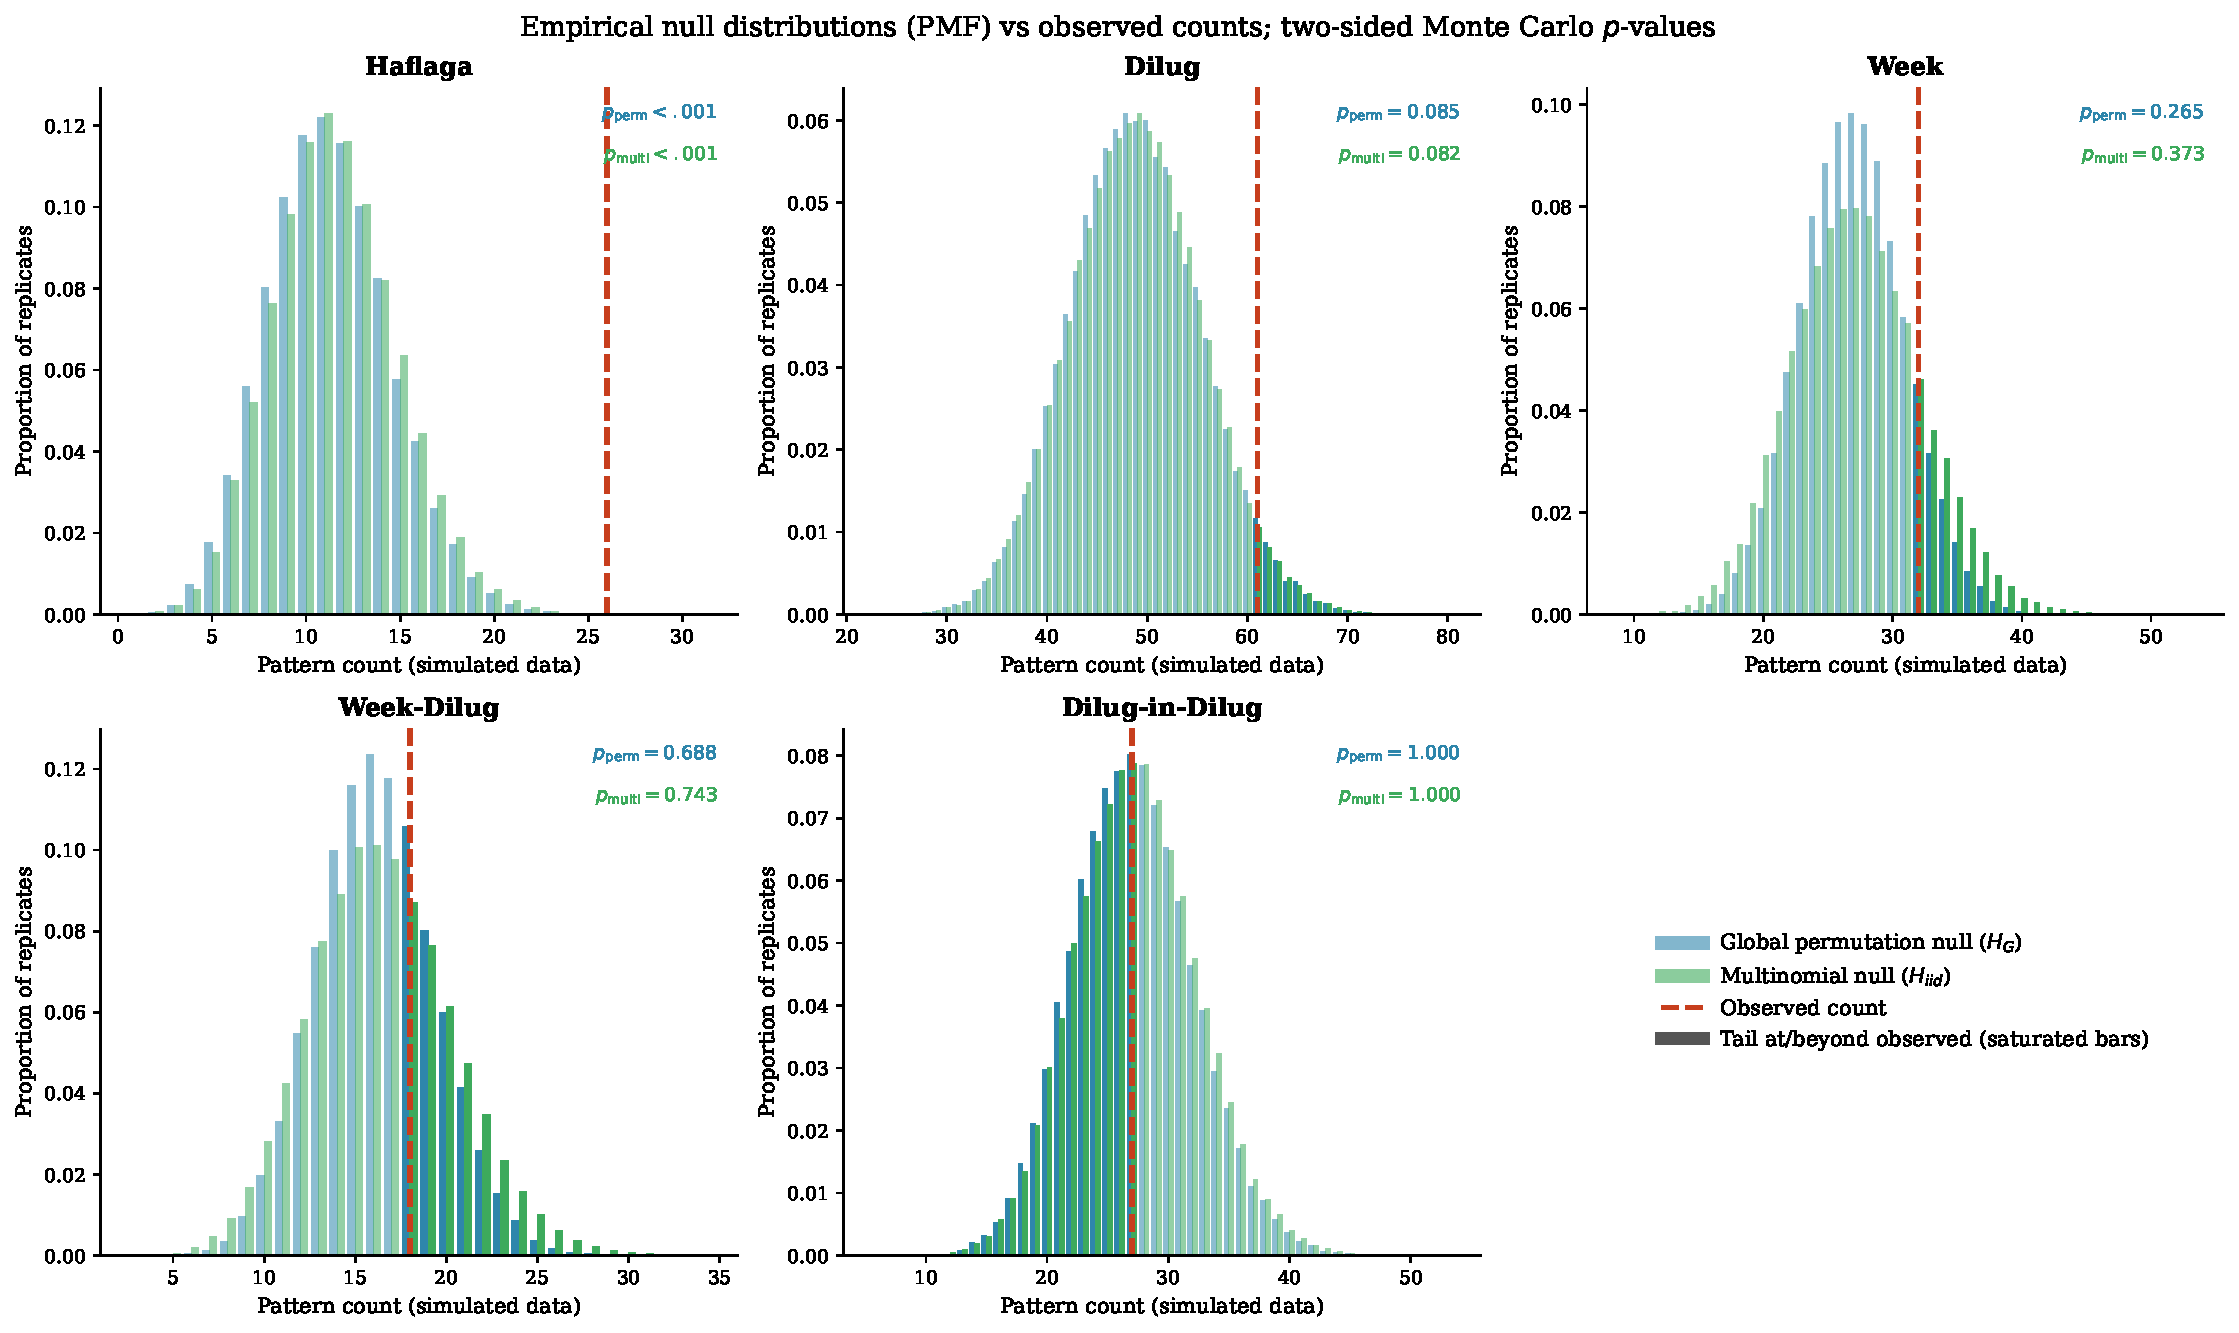
\includegraphics[width=\textwidth]{fig3_null_distributions}
  \caption{Empirical null probability mass functions under $\HG$ (left bar of each
    pair) and $\HI$ (right bar) with the observed count (dashed line). Saturated bars mark
    the tail at or beyond the observed count on the observed side; the two-sided $p$-value
    is twice the smaller tail probability (Eq.~\ref{eq:ptwo}) and is printed in each
    panel for both nulls.}
  \label{fig:nulldists}
\end{figure}

\begin{figure}[!htbp]
  \centering
  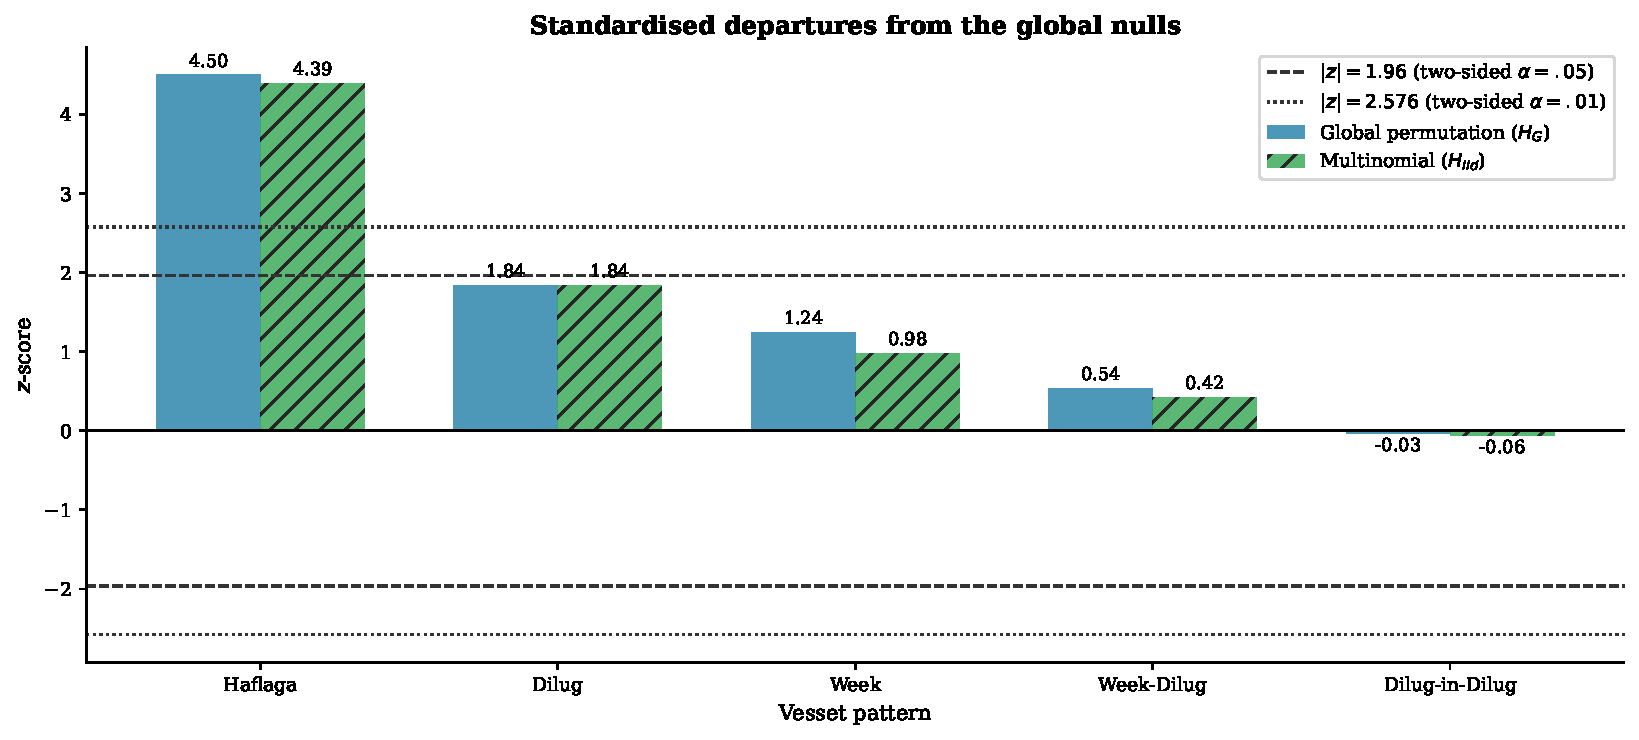
\includegraphics[width=0.88\textwidth]{fig4_zscores}
  \caption{Standardised departures $z_j$ under $\HG$ (solid) and $\HI$ (hatched).
    Dashed and dotted lines mark $|z| = 1.96$ and $2.576$. The two nulls give different
    $z$ for the same count because each has its own mean and SD (e.g.\ Week: 1.24 vs.\
    0.98).}
  \label{fig:zscores}
\end{figure}

\begin{figure}[!htbp]
  \centering
  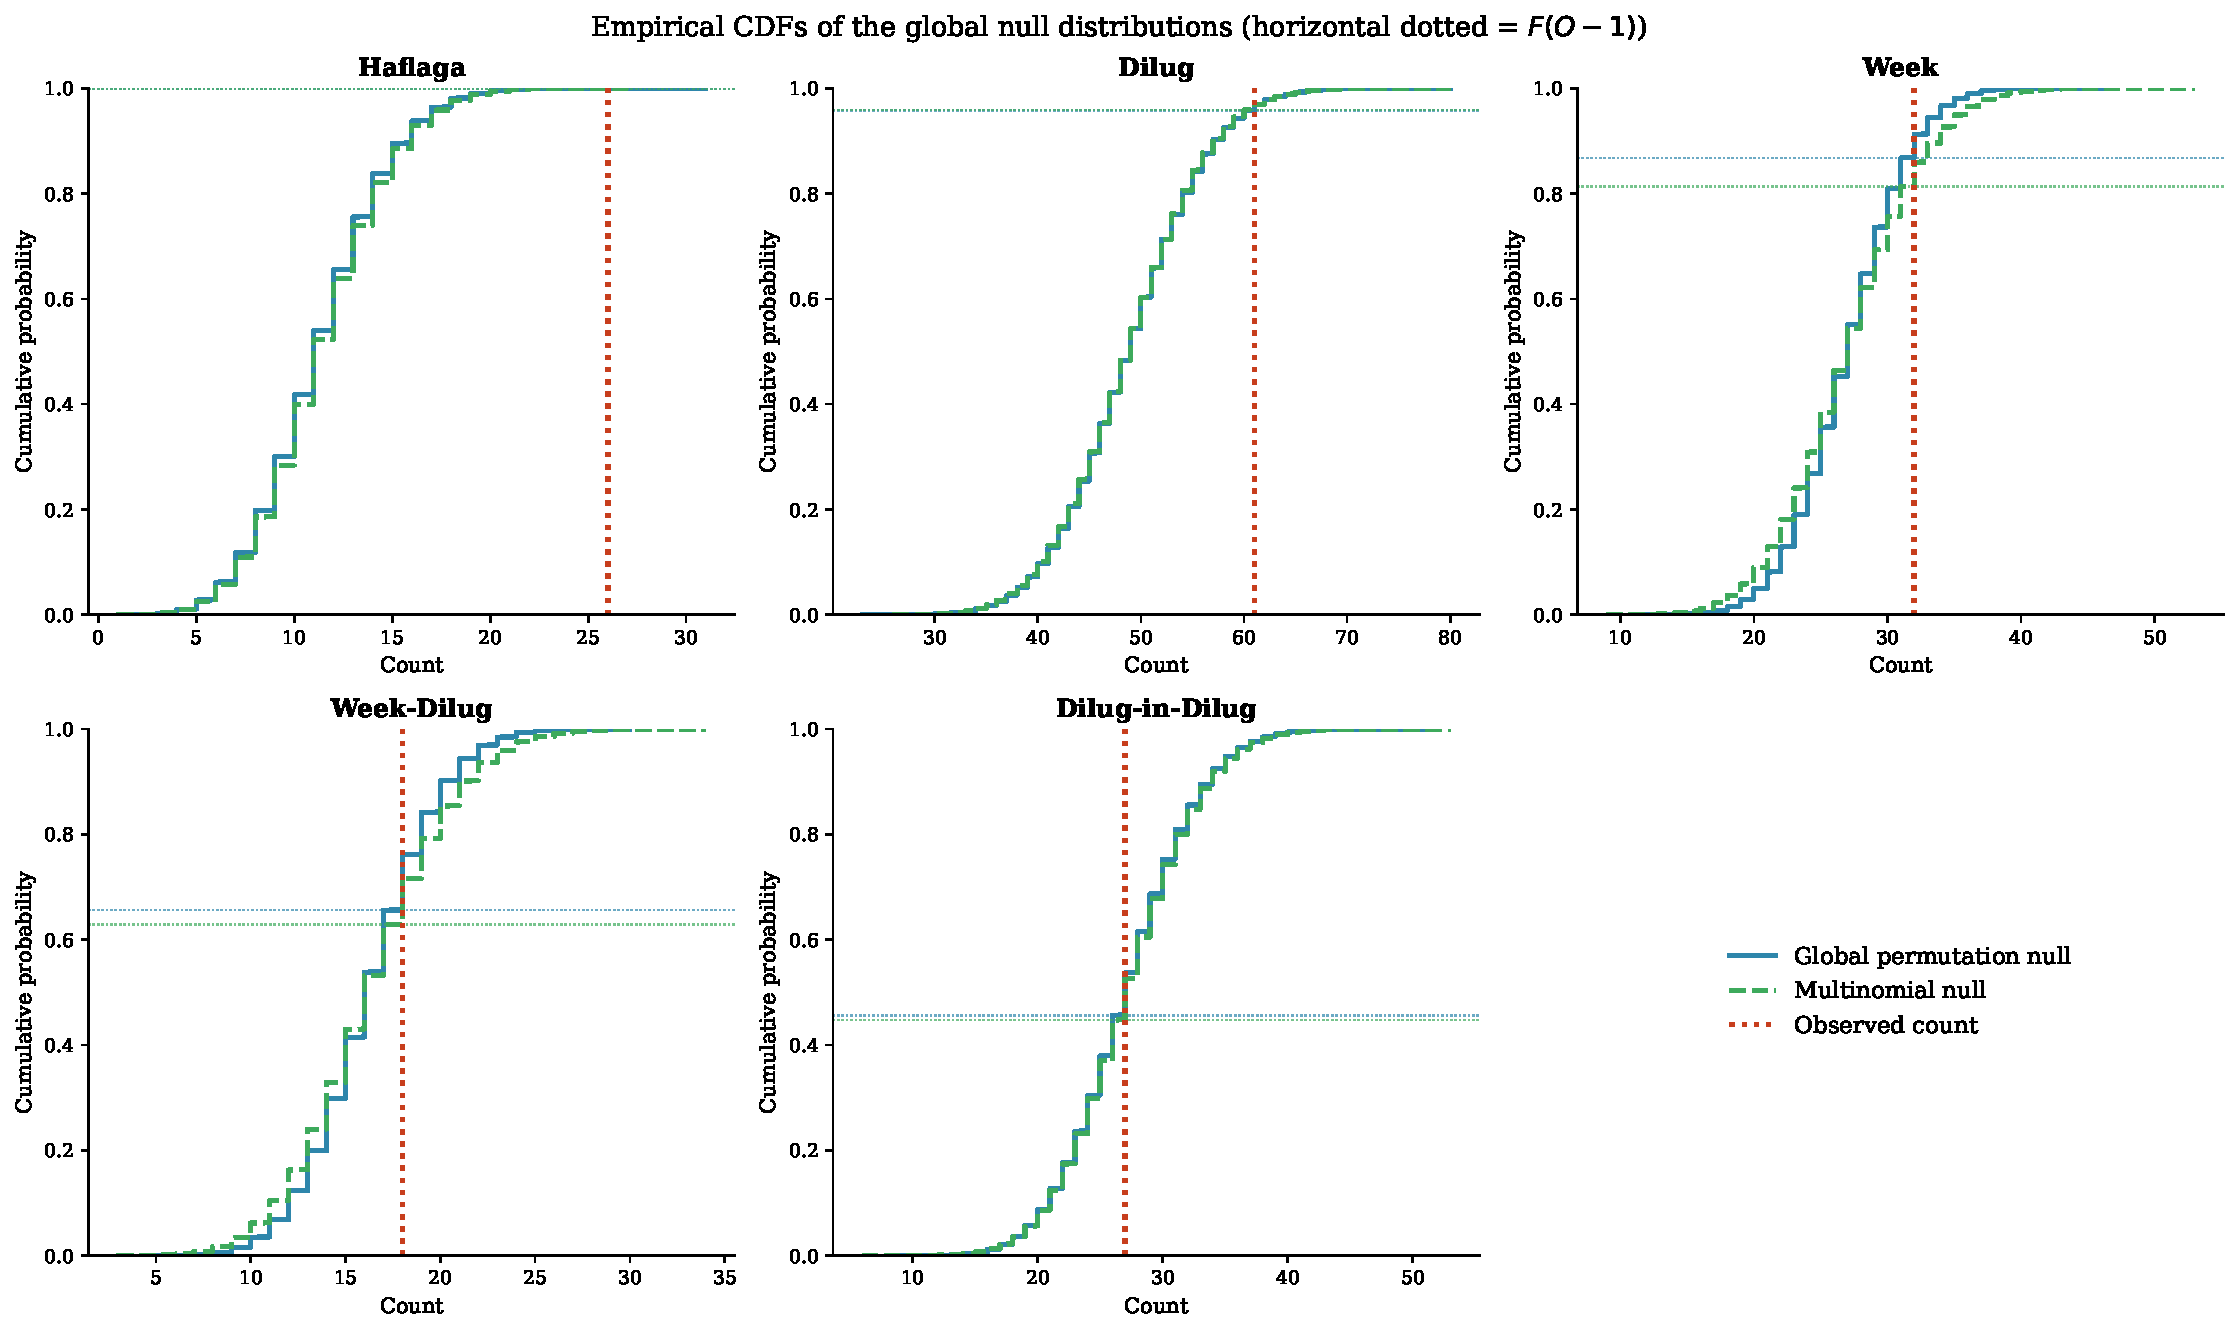
\includegraphics[width=\textwidth]{fig5_cdfs}
  \caption{Empirical CDFs of the $\HG$ (solid) and $\HI$ (dashed) null distributions;
    dotted vertical line at the observed count.}
  \label{fig:cdfs}
\end{figure}

\subsection{Within-Woman Null}
\label{sec:stratified}

The global nulls remove between-woman heterogeneity in regularity: they ask whether the
counts exceed what a homogeneous population would produce, not whether each woman's
\emph{ordering} produces events beyond what her own values predict. $\HW$ asks the
latter. Table~\ref{tab:stratified} and Figure~\ref{fig:stratified} give the results.

\begin{table}[!htbp]
\centering
\caption{Within-woman permutation null $\HW$ ($B = 50{,}000$; all 118 women; each
  woman's sequence permuted without replacement). $p$-values are two-sided
  (Eq.~\ref{eq:ptwo}); Holm adjustment across the five patterns. LOO range: range of the
  two-sided $p$-value over the 118 leave-one-woman-out analyses.}
\label{tab:stratified}
\smallskip
\begin{tabular}{L{2.9cm} C{1.0cm} C{1.4cm} C{1.2cm} C{1.2cm} C{1.2cm} C{1.2cm} C{2.0cm}}
\toprule
\textbf{Pattern} & \textbf{Obs.} & \textbf{Null mean} & \textbf{Null SD}
  & $\mathbf{z}$ & $\mathbf{p}$ & \textbf{Holm} & \textbf{LOO range} \\
\midrule
Haflaga        & 26 & 31.84 & 4.68 & $-1.25$ & $.254$ & $1.00$ & $.12$--$.39$ \\
Dilug          & 61 & 67.04 & 7.38 & $-0.82$ & $.460$ & $1.00$ & $.34$--$.60$ \\
Week           & 32 & 33.79 & 3.88 & $-0.46$ & $.749$ & $1.00$ & $.53$--$.93$ \\
Week-Dilug     & 18 & 20.91 & 3.22 & $-0.90$ & $.460$ & $1.00$ & $.31$--$.69$ \\
Dilug-in-Dilug & 27 & 39.12 & 5.84 & $-2.07$ & $.038$ & $.192$ & $.014$--$.073$ \\
\midrule
\multicolumn{8}{@{}p{14.6cm}@{}}{Joint test (five patterns): $\DM = 2.93$, $p = .126$ (6,285 of 50,000 replicates at or beyond the observed value); split-batch $\DM = 2.95$, $p = .119$; leave-one-woman-out range of $p$: $.055$--$.224$.} \\
\bottomrule
\end{tabular}
\end{table}

Under $\HW$ no pattern is significant after Holm correction, and all five observed
counts lie \emph{below} their conditional null means. The most extreme component is
Dilug-in-Dilug ($z = -2.07$; nominal two-sided $p = .038$, Holm $p = .19$): fewer
second-order progressions were observed than random reorderings of the same values
produce. The direction is noted; the mechanism is not identified by these data, and the
result is exploratory. The joint test is non-significant ($\DM = 2.93$, $p = .13$) and
essentially unchanged in the split-batch form ($\DM = 2.95$, $p = .12$).

The shift between nulls is large: for Haflaga the $\HG$ null is centred at 11.3 and the
$\HW$ null at 31.8, above the observed 26. A principal contributor to this shift is that
women with narrow cycle-length multisets generate many exact repetitions under
\emph{any} ordering of their values; conditioning on each woman's multiset preserves this
feature, whereas the global nulls erase it.

\begin{figure}[!htbp]
  \centering
  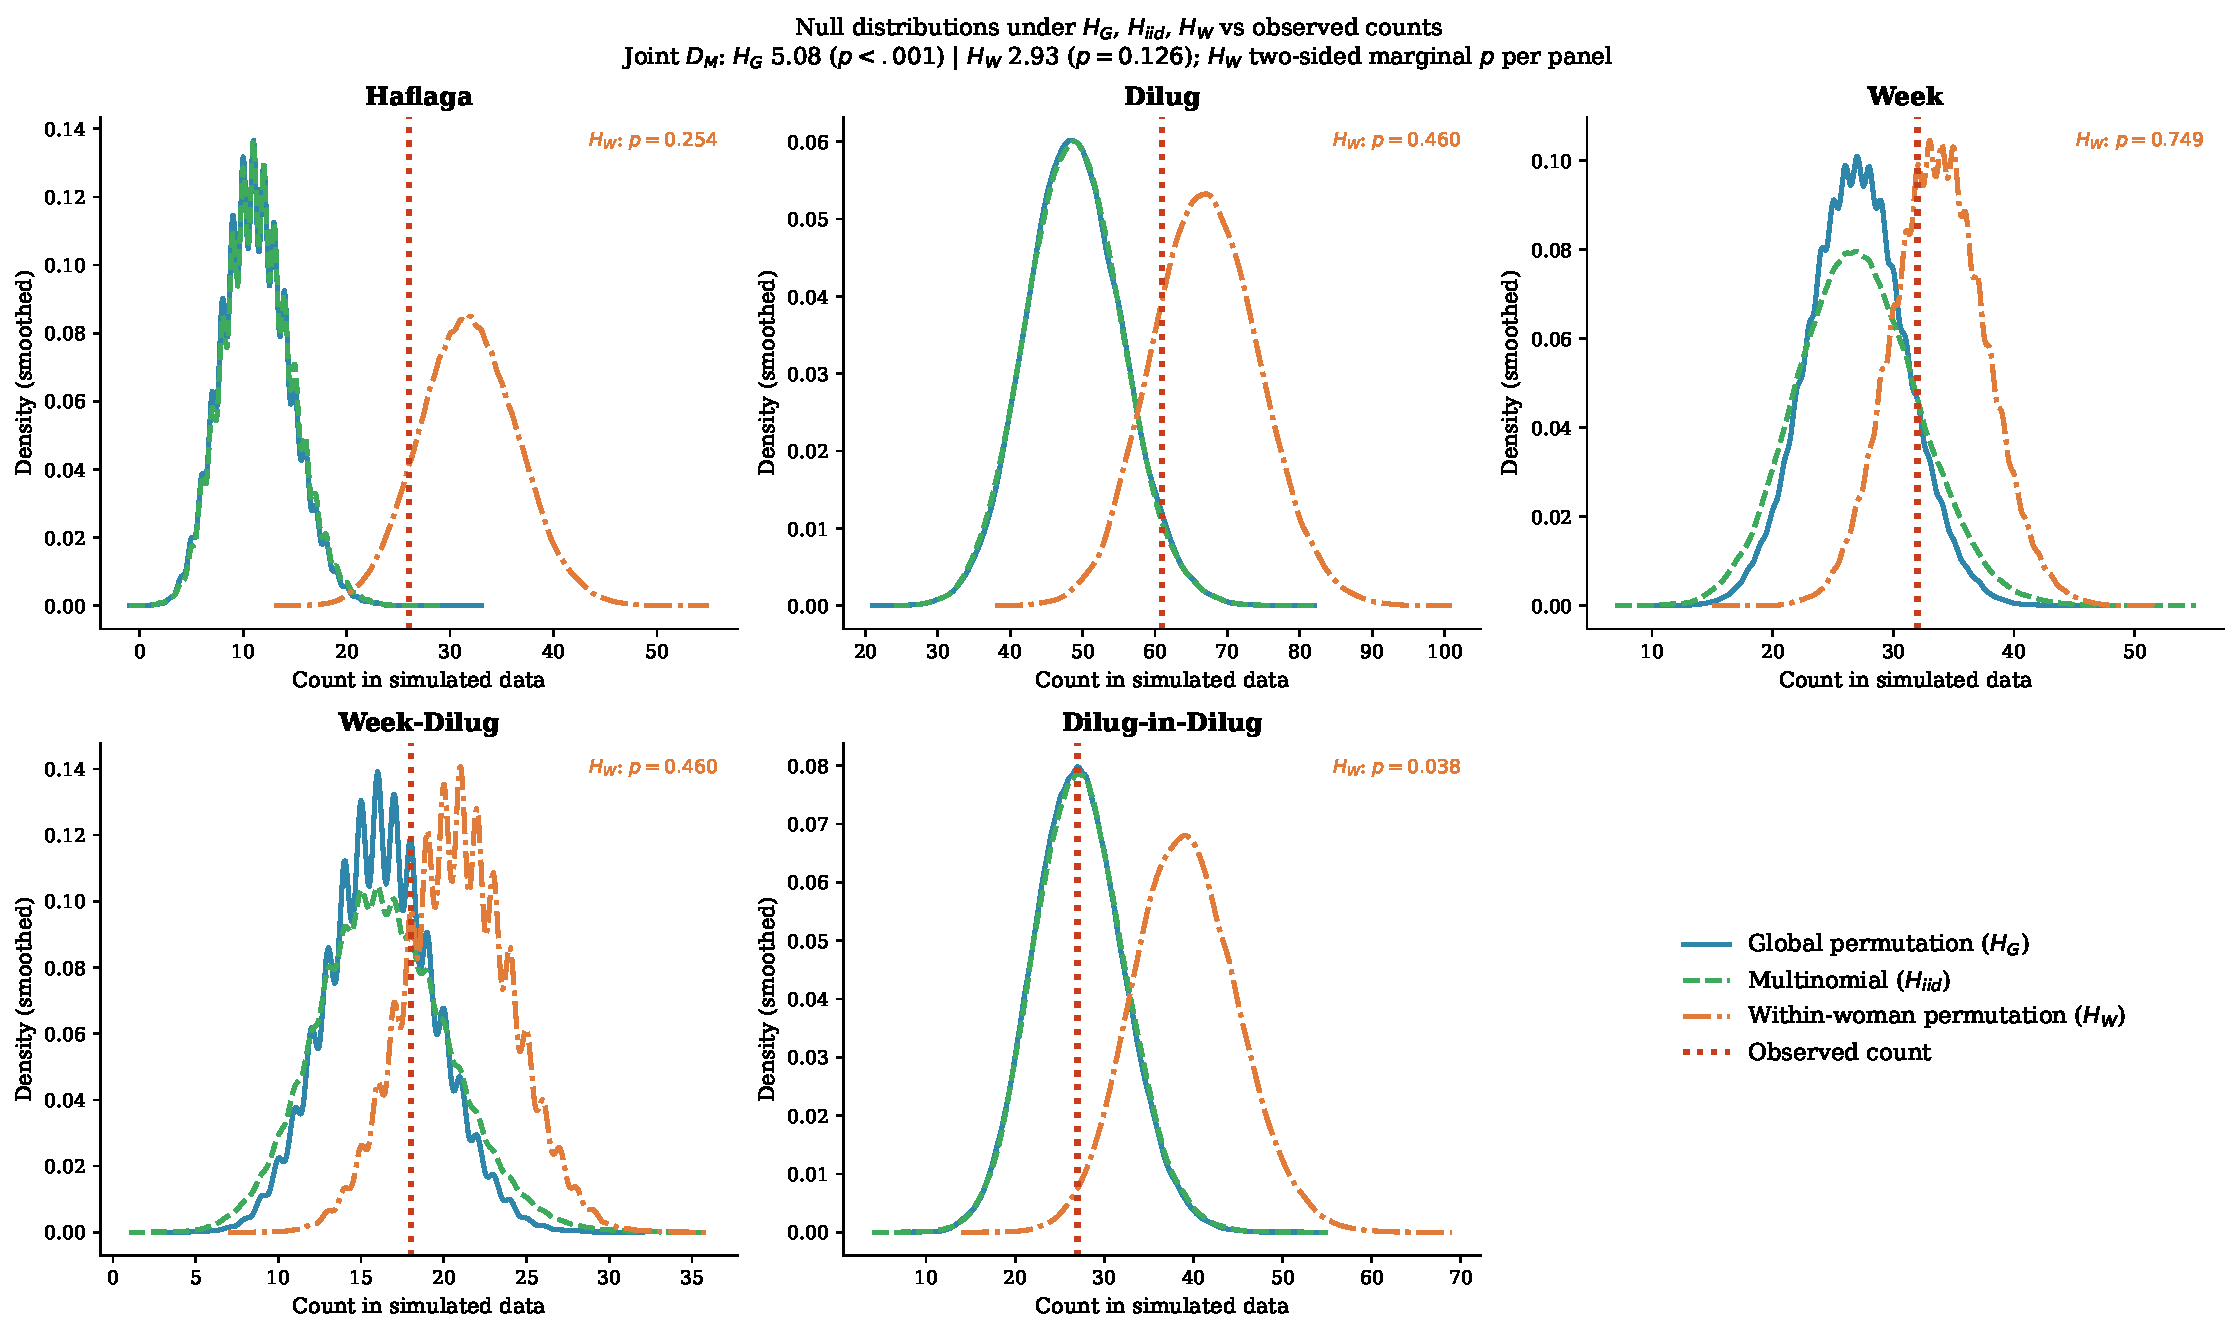
\includegraphics[width=\textwidth]{fig6_stratified_comparison}
  \caption{Smoothed null densities (for visual comparison only; inference uses the
    empirical PMFs) under $\HG$ (solid), $\HI$ (dashed) and $\HW$ (dash-dotted) for each
    pattern, with the observed count (dotted vertical line) and the two-sided $\HW$
    $p$-value in each panel.}
  \label{fig:stratified}
\end{figure}

\subsection{Joint Tests}
\label{sec:joint}

Under $\HG$ the five-pattern Mahalanobis distance is $\DM = 5.08$ ($p < .001$; 6 of
50,000 replicates at or beyond) and under $\HI$ it is $\DM = 4.87$ ($p < .001$; 17 of
50,000); the split-batch values are $5.07$ and $4.87$ with the same $p$-values. Under
$\HW$, $\DM = 2.93$, $p = .126$ (Table~\ref{tab:stratified};
Figure~\ref{fig:joint1d}). The displacement under the global nulls is driven by Haflaga,
which has the smallest null SD (3.27) and the largest standardised departure and
therefore receives the largest weight in the quadratic form; the null covariance matrices
are well conditioned (condition numbers 4.6, 4.4 and 5.4 for $\HG$, $\HI$, $\HW$) with
all pairwise null correlations below 0.17 in absolute value.

The exploratory three-pattern test (Haflaga, Week-Dilug, Dilug-in-Dilug) gives
$\DM = 4.50$ ($p < .001$), $4.39$ ($p < .001$) and $2.68$ ($p = .067$) under $\HG$,
$\HI$ and $\HW$ respectively, consistent with the five-pattern analysis
(Figure~\ref{fig:joint3panels}).

\begin{figure}[!htbp]
  \centering
  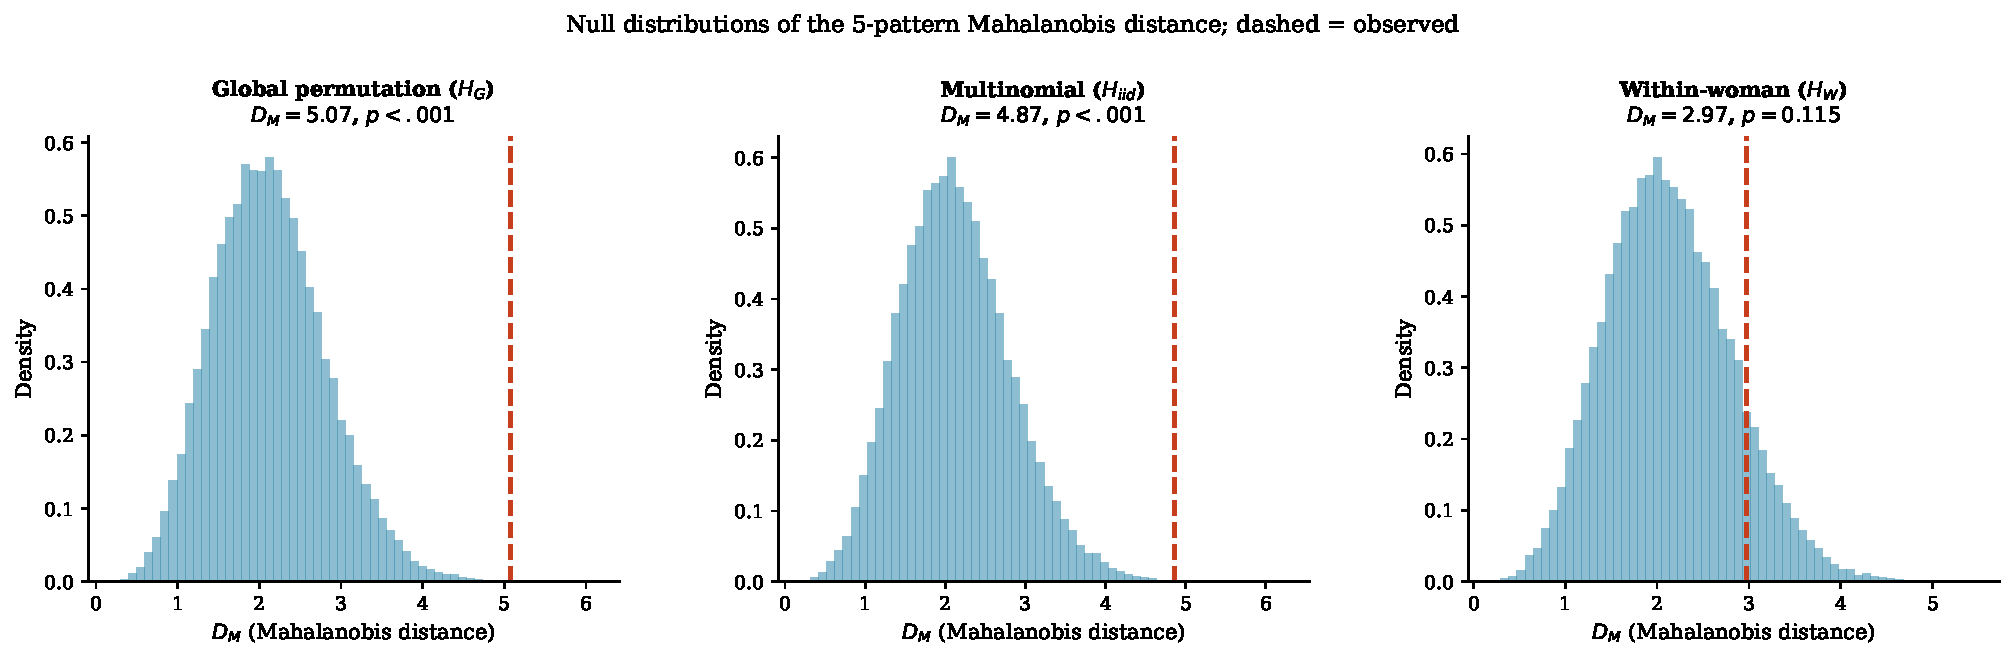
\includegraphics[width=\textwidth]{fig7_dm_nulldist}
  \caption{Null distributions of the five-pattern Mahalanobis distance $\DM$
    (Eq.~\ref{eq:mahalanobis}) under $\HG$ (left), $\HI$ (centre) and $\HW$ (right);
    dashed line at the observed value.}
  \label{fig:joint1d}
\end{figure}

\begin{figure}[!htbp]
  \centering
  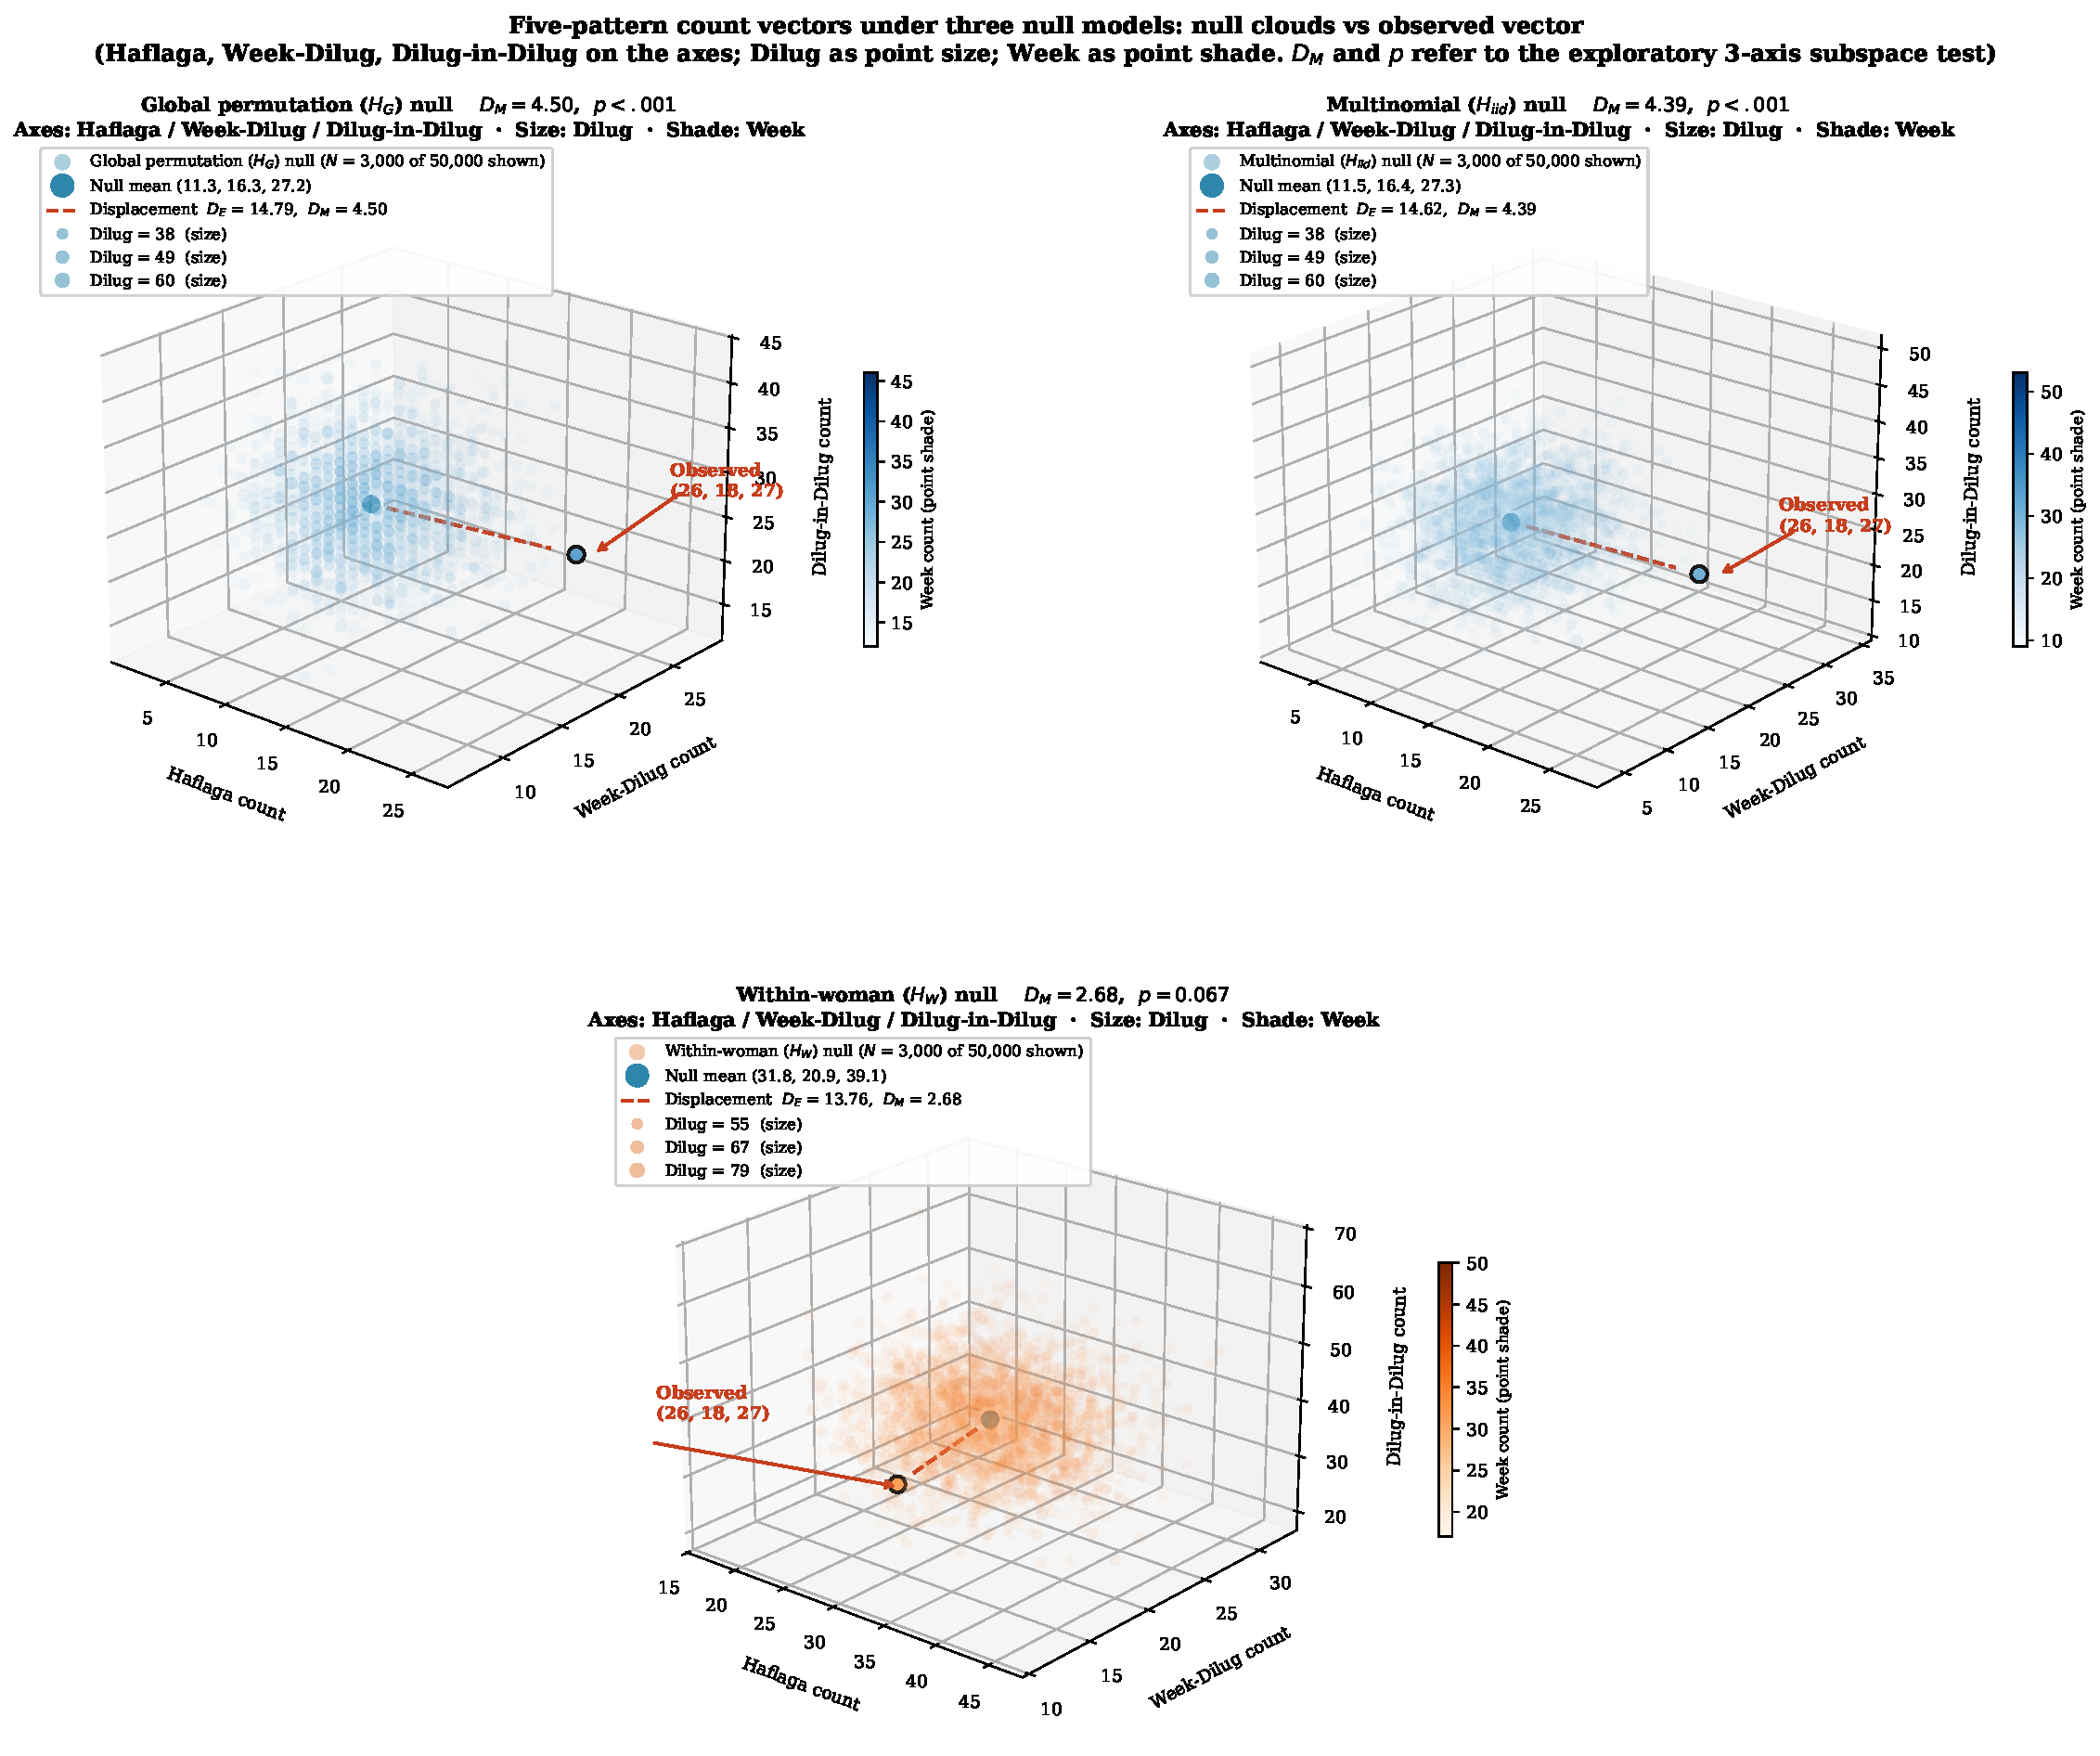
\includegraphics[width=\textwidth]{fig9_joint_3panels}
  \caption{Five-pattern count vectors under the three null models: 3,000 of the 50,000
    null replicates (points) and the observed vector under $\HG$ (top left), $\HI$ (top
    right) and $\HW$ (bottom). All five counts are shown for every replicate: Haflaga,
    Week-Dilug and Dilug-in-Dilug on the axes, Dilug as marker size (size legend in each
    panel) and Week as marker shade (colour bar). The filled circle is the null mean and
    the dashed segment the displacement to the observed vector $(26, 18, 27)$ on the
    three axes; the $D_E$ and $D_M$ values in the legends and titles are those of the
    exploratory three-axis subspace test (Section~\ref{sec:joint}). Primary inference
    uses the five-pattern $\DM$ (Table~\ref{tab:stratified}).}
  \label{fig:joint3panels}
\end{figure}

\subsection{Pairwise Dependence (Exploratory; Supporting Information)}
\label{sec:chisq}

The exploratory between-woman pairwise analysis (Supporting Information, Section~S1,
Table~S1, Figure~S1) is consistent with the relationships of Section~\ref{sec:mathdep}:
of the ten pairs, only Haflaga $\times$ Dilug-in-Dilug survives Holm correction
($r_s = 0.27$, permutation $p = .004$, Holm $p = .038$), Haflaga $\times$ Week-Dilug is
positive as containment requires but does not survive ($r_s = 0.23$, Holm $p = .10$),
and the remaining eight pairs are null. The binary ever/never version and a permutation
stratified by follow-up length give the same ordering and essentially the same $p$-values.
These associations are between women, not within sequences; they say nothing about
temporal ordering and are compatible with, not evidence for, the proximity argument.

\subsection{Simulation Validation and Sensitivity}
\label{sec:simresults}

\paragraph{Size.}
Table~\ref{tab:size} reports empirical rejection rates under each null for 10,000 fresh
pseudo-observed datasets (Monte Carlo standard error about 0.002 at $\alpha = .05$).
Type-I error is controlled at or below the nominal level by the marginal and Holm
procedures and is approximately nominal for the joint test: the two-sided marginal tests
reject between 2.9\% and 4.8\% of the time (conservative because the counts are
discrete), the Holm family between 3.2\% and 3.7\%, and the joint test between 4.8\% and
5.3\% at $\alpha = .05$ and between 0.7\% and 1.1\% at $\alpha = .01$. The plug-in and
split-batch versions of the joint test are indistinguishable, so re-using the replicates
for $\hat\Sigma$ has no detectable effect at $B \geq 20{,}000$.

\begin{table}[!htbp]
\centering
\caption{Empirical size at nominal $\alpha = .05$ (10,000 pseudo-observed datasets per
  null, each tested against an independent batch of 20,000 replicates). Joint test shown
  in plug-in form ($\hat\Sigma$ and reference distribution from the same batch) and
  split-batch form; values at $\alpha = .01$ in parentheses.}
\label{tab:size}
\smallskip
\small
\begin{tabular}{l C{1.1cm} C{1.1cm} C{1.1cm} C{1.1cm} C{1.1cm} C{1.3cm} C{1.9cm} C{1.9cm}}
\toprule
& \multicolumn{5}{c}{Marginal two-sided tests} & Holm & \multicolumn{2}{c}{Joint $\DM$} \\
\cmidrule(lr){2-6}\cmidrule(lr){8-9}
Null & Haf. & Dilug & Week & W-D & DiD & family & plug-in & split-batch \\
\midrule
$\HG$  & .029 & .047 & .034 & .031 & .046 & .033 & .048 (.011) & .052 (.010) \\
$\HI$  & .048 & .038 & .040 & .038 & .046 & .032 & .049 (.007) & .047 (.007) \\
$\HW$  & .043 & .041 & .043 & .042 & .040 & .037 & .053 (.009) & .053 (.010) \\
\bottomrule
\end{tabular}
\end{table}

\paragraph{Power of the within-woman tests.}
Table~\ref{tab:power} and Figure~\ref{fig:power} give rejection rates of the $\HW$ tests
for datasets with genuine within-woman ordering (400 datasets per scenario; Monte Carlo
SE $\leq 0.025$). At $\rho = 0$ and $q = 0$, which are exchangeable within woman, all
tests reject at nominal rates under these heterogeneous marginals (joint 6.2\%, SE 1.2\%).
Autoregressive dependence with $\rho = 0.25$ --- which raises the expected Haflaga count
by about five events over its conditional null mean --- is detected by the joint test in
51\% of datasets and by the Holm family in 26\%; at $\rho = 0.5$ the joint test rejects
in 99.5\% and at $\rho = 0.75$ always. Exact-repetition persistence is detected far more
readily: when one cycle in ten copies its predecessor ($q = 0.1$) the joint test rejects
in 98\% of datasets and the Haflaga marginal test in 96\%; at $q \geq 0.2$ detection is
certain. The Dilug-in-Dilug marginal has no power against persistence (repetition
suppresses second-order progressions), and Week-Dilug has the least power against
autoregression, as expected from their definitions.

\begin{table}[!htbp]
\centering
\caption{Power of the $\HW$ tests at $\alpha = .05$ against within-woman
  temporal-dependence alternatives (400 datasets per scenario, each analysed with its own
  2,000 within-woman permutations). $\Delta$Haf.: mean observed Haflaga count minus its
  mean conditional null expectation. The $\rho = 0$ and $q = 0$ rows are exchangeable
  within woman and serve as size checks.}
\label{tab:power}
\smallskip
\small
\begin{tabular}{l C{1.0cm} C{1.2cm} C{1.0cm} C{1.0cm} C{1.0cm} C{1.0cm} C{1.0cm} C{1.2cm} C{1.2cm}}
\toprule
Alternative & Level & $\Delta$Haf. & Haf. & Dilug & Week & W-D & DiD & Holm & Joint \\
\midrule
AR(1) $\rho$       & 0    & $-0.1$ & .04 & .05 & .04 & .04 & .04 & .03 & .06 \\
                   & 0.25 & $+5.1$ & .18 & .24 & .10 & .06 & .18 & .26 & .51 \\
                   & 0.50 & $+13.8$ & .76 & .74 & .35 & .31 & .44 & .89 & .995 \\
                   & 0.75 & $+33.3$ & 1.00 & .97 & .78 & .66 & .73 & 1.00 & 1.00 \\
\midrule
Persistence $q$    & 0    & $+0.2$ & .04 & .04 & .04 & .04 & .06 & .05 & .06 \\
                   & 0.1  & $+24.1$ & .96 & .19 & .61 & .41 & .04 & .94 & .98 \\
                   & 0.2  & $+52.7$ & 1.00 & .60 & .96 & .86 & .04 & 1.00 & 1.00 \\
                   & 0.3  & $+80.4$ & 1.00 & .93 & .99 & .96 & .16 & 1.00 & 1.00 \\
\bottomrule
\end{tabular}
\end{table}

\begin{figure}[!htbp]
  \centering
  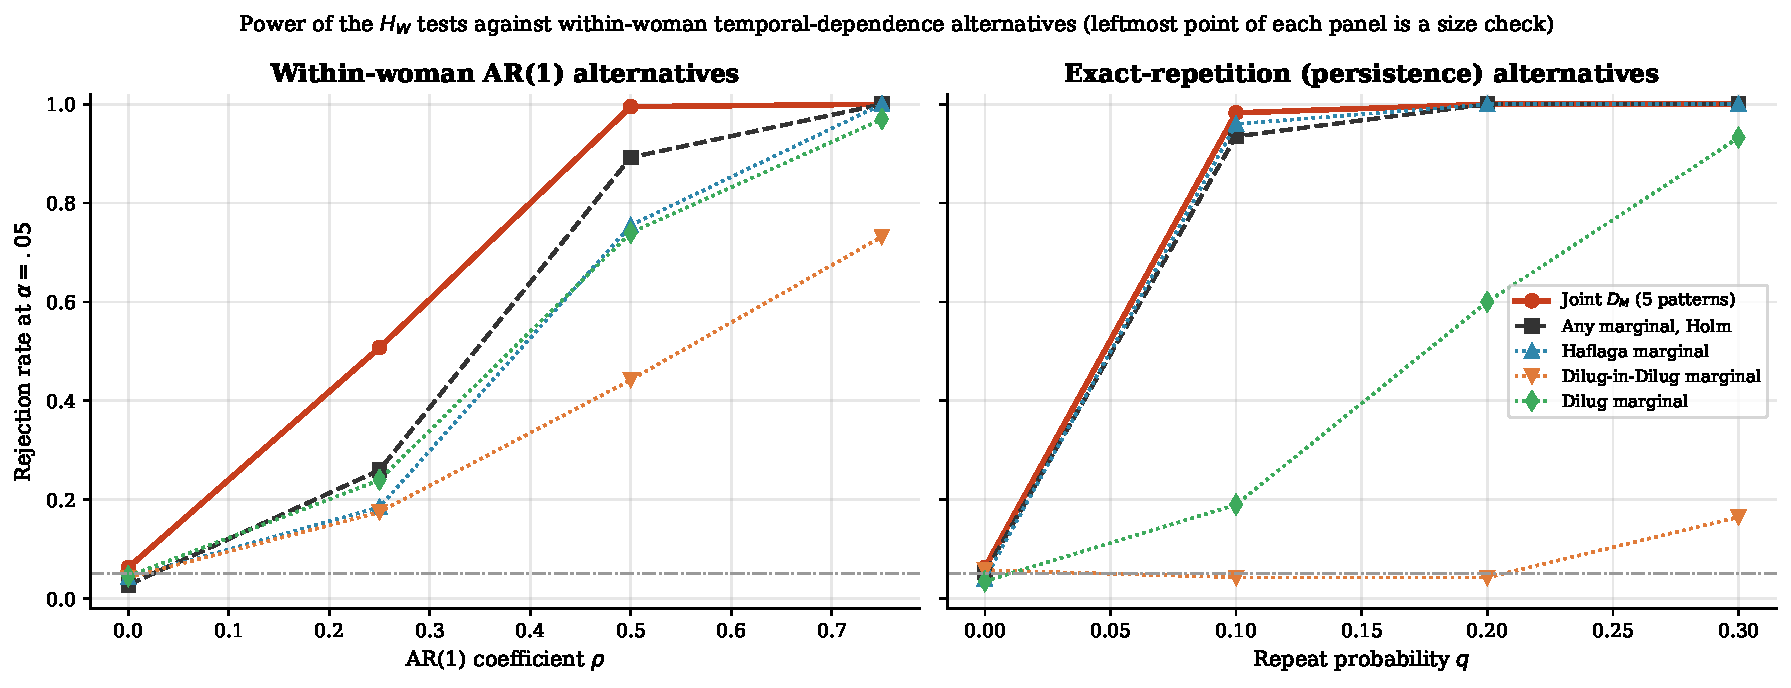
\includegraphics[width=\textwidth]{fig10_power}
  \caption{Rejection rates of the $\HW$ tests at $\alpha = .05$ against within-woman
    AR(1) alternatives (left) and exact-repetition alternatives (right); the leftmost
    point of each panel is a size check. Solid: joint five-pattern $\DM$; dashed: any
    Holm-corrected marginal; dotted: selected marginal tests. Dash-dotted horizontal line
    at 0.05.}
  \label{fig:power}
\end{figure}

These results calibrate the main finding for the two mechanisms simulated. Under the
AR(1) alternative at $\rho = 0.25$, which added about five Haflaga events on average,
the joint test rejected in 51\% of datasets; at $\rho = 0.5$ (about 14 additional
events) it rejected in 99.5\%. Under the persistence alternative, one exact repetition
in ten cycles was detected in 98\% of datasets. The observed Haflaga count is six
\emph{below} its conditional null mean. These figures do not transfer to arbitrary forms
of temporal dependence: autoregression weaker than $\rho \approx 0.25$, or dependence
that does not manifest as whole-day autoregression or exact repetition, may go
undetected by these statistics.

\paragraph{Sensitivity to unequal follow-up.}
Eleven women with 20 or more cycles contribute 20\% of cycles and 35\% of Haflaga events
(21\%, 28\%, 11\% and 30\% of Dilug, Week, Week-Dilug and Dilug-in-Dilug events); the
Spearman correlation between a woman's cycle count and her Haflaga events is 0.28. When
every woman is truncated to her first 12 cycles (1,289 cycles), the observed counts are
$(19, 51, 21, 16, 21)$, all $z$ remain negative ($-1.18$, $-0.32$, $-0.89$, $-0.68$,
$-1.78$), no marginal test approaches significance (smallest two-sided $p = .080$, for
Dilug-in-Dilug), and the joint test gives $\DM = 2.49$, $p = .29$. Leaving out any single
woman moves the joint $\HW$ $p$-value within $.055$--$.224$ and never below $.05$
(Table~\ref{tab:stratified}); the nominal Dilug-in-Dilug marginal stays below $.05$ in
114 of 118 leave-one-out analyses, so it is not driven by one woman, but it remains
non-significant after Holm correction throughout.

% ─── 5. Discussion ────────────────────────────────────────────────────────────
\section{Discussion}

\subsection{What the Contrast Between Nulls Shows}

The same five counts are extreme under population-level exchangeability
($\DM = 5.08$, $p < .001$) and unremarkable under within-woman exchangeability
($\DM = 2.93$, $p = .13$). The global result is real and is not an artefact of the
multinomial versus permutation choice (the two agree). It says that vesset events are
concentrated in a way a homogeneous population would not produce. The within-woman result
says that, conditional on each woman's own cycle-length values, the order in which they
occurred produced no detectable excess of rule-defined events --- for these exact
statistics, against random reorderings, at the sensitivity documented in
Section~\ref{sec:simresults}. The simplest account consistent with both is
between-woman heterogeneity in regularity: women with narrow cycle-length distributions
generate many exact repetitions under any ordering, and the global nulls, which pool
across women, treat this as excess. This account is supported by the data; it is not
uniquely identified by them, and other mechanisms that leave the multiset-conditional
distribution of these counts unchanged cannot be excluded.

Two things the $\HW$ result does not show should be stated. It does not show that cycle
lengths are serially independent: the autocorrelation documented by \citet{ecochard2024}
in an overlapping cohort is exactly the kind of structure that $\HW$ destroys, and its
non-detection here means only that it does not translate into extra exact vesset events
in this sample. And it does not show that the rules are without anticipatory value:
whether a woman with three equal consecutive intervals is more likely to repeat the
interval is a forecasting question, not addressed here.

\subsection{Primary, Exploratory and Robustness Analyses}

\emph{Primary:} the five-pattern joint tests under $\HG$ and $\HW$, and the Holm-corrected
marginal tests under each. \emph{Exploratory:} the Dilug marginal ($p = .085$), the
Dilug-in-Dilug deficit under $\HW$ (Holm $p = .19$), the pairwise associations
(Supporting Information), and the three-pattern subspace. \emph{Robustness:} the multinomial null, the split-batch joint
test, truncation, and leave-one-woman-out. No analysis was pre-registered; the
five-pattern family was fixed after two rules were found to have zero occurrences
(Section~\ref{sec:data}).

\subsection{Pattern-Specific Findings}

Haflaga is the only pattern that departs from a global null after multiplicity control
and it does so strongly (4 of 50,000 replicates reached the observed count). Under $\HW$
its count is below the conditional mean. The 20 women with Haflaga events have markedly
lower within-woman SD than women with no events, as the definition of the rule implies;
this characterises whom the rule selects rather than validating it. Dilug's global
$z = 1.84$ does not survive correction and should be treated as hypothesis-generating;
gradual trends (age, weight, hormonal change) would produce arithmetic progressions,
but no such mechanism is tested here. The Week pattern in this sample is almost entirely
the 28-day cycle (haflaga 29) repeated twice, because longer weekly anchors (35, 42 days)
are rare (9.6\% of cycles are $\geq 35$ days). Week-Dilug events include the 3 Haflaga-30
sequences by containment.

\subsection{The Joint Statistic}

The quadratic form standardises each component by its null variance and accounts for
the null covariance implied by the definitions; Haflaga dominates under the global nulls
because its null SD is smallest. Hotelling's $T^2$ shares the form but assumes
multivariate normality of the count vector, which fails for counts as small as 18; the
Monte Carlo reference distribution avoids this. A max-$T$ statistic would be less
sensitive to simultaneous displacement of several components; in these data it leads to
the same conclusions under all nulls. Using the same replicates to estimate $\hat\Sigma$
and to form the reference distribution introduces a finite-$B$ dependence; the
split-batch results and the size simulation show it is immaterial at $B = 50{,}000$. We
regard the statistic as a routine adaptation of permutation MANOVA-type tests
\citep{anderson2001} to rule-defined counts and claim nothing further for it.

\subsection{Implications}

All implications are hypotheses for future study; none is tested here. A woman with an
established Haflaga has a within-woman SD below about 1.6 days in this dataset, which is
the situation in which calendar-based fertility awareness is most reliable
\citep{bortot2010}; whether the halachic marker adds to statistical cycle-length
prediction is the subject of a companion forecasting study \citep{ross_planned}. For
observant Jewish women the within-woman result is consistent with the traditional
understanding that the rules codify observed regularity; whether the empirical findings
bear on the legal standing of the rules is outside the scope of statistics. Changes in
vesset status could in principle signal a change in regularity, a clinical hypothesis
that would require datasets with clinical endpoints.

\subsection{Transferable Lesson}

The reusable content of this case is not the statistic but the null-model comparison.
Whenever deterministic rules are applied to recurrent-event sequences from many subjects
with unequal follow-up --- exact inter-seizure intervals in epilepsy diaries, repeated
inter-episode intervals in mood disorders, fixed-lag repetitions in behavioural logs ---
a pooled or i.i.d.\ null confounds between-subject heterogeneity with within-subject
structure, and a within-subject permutation null conditional on each subject's observed
multiset isolates the ordering question at the cost of answering only that question. The
two should be reported together, with a simulation showing what the conditional test can
detect. Only within-subject data with a defined generative alternative could sharpen this
further; a parametric null from a fitted state-space model \citep{bortot2010} would be a
natural next step.

\subsection{Limitations}
\label{sec:limitations}

\paragraph{Coding and measurement.}
Counts are invariant to the $H_k = L_k + 1$ relabelling provided the Week-Dilug anchor is
shifted accordingly (verified: 26 Haflaga, 18 Week-Dilug under both conventions;
computing on $L_k$ with an unshifted anchor of 30 gives 12 Week-Dilug events). The
haflaga distribution declines smoothly through the anchor ($H = 29$: 225 cycles;
$30$: 175; $31$: 141; Figure~\ref{fig:heaping}), so the Week-Dilug count does not appear
to reflect digit preference; no formal test of heaping was performed. Onset time of day
is not recorded, so some events may be misclassified relative to the halachic requirement
of a common onset period; a shift that is constant within a woman leaves her multiset and
hence the $\HW$ analysis unchanged, but shifts that vary within a woman are not
addressed.

\paragraph{Scope.}
Calendar dates are absent, precluding the 10 date-dependent rule types; body-sign
patterns (\textit{vesset haguf}) are invisible to cycle-length data. The two
repeating-cycle rules were not analysed after zero occurrences were observed
(Section~\ref{sec:data}). The sample consists of non-Jewish, regularly cycling, married
NFP users (trial eligibility 18--42 years; \citealp{fehring2013}), a self-selected,
cycle-aware group who may be more regular than
the general population; some halachic authorities hold that regularities in this
population need not transfer to observant Jewish women \citep{ross2022phd}. Results
should not be generalised without replication in the target population.

\paragraph{Statistical.}
$\HW$ tests exchangeability of each woman's observed values and nothing more general.
The simulations (Section~\ref{sec:simresults}) show high power against the simulated
exact-repetition mechanism and against simulated whole-day AR(1) dependence of moderate
strength ($\rho \geq 0.5$), about 50\% power at $\rho = 0.25$, and, necessarily, none
against dependence that leaves the distribution of these exact count statistics
unchanged; the non-rejection should be read with those limits. The aggregate-count
estimand weights women by follow-up; the truncation and leave-one-woman-out analyses
indicate that this does not drive the conclusions. The archived file contains no cycle
shorter than 18 or longer than 54 days, so any restriction of cycle length was applied
upstream of the released data and its effect cannot be assessed here. The exploratory pairwise associations (Supporting Information) involve
rare patterns (18 and 27 events), rest on few women, and remain exposed to residual
dependence of both rates on follow-up length.

\begin{figure}[!htbp]
  \centering
  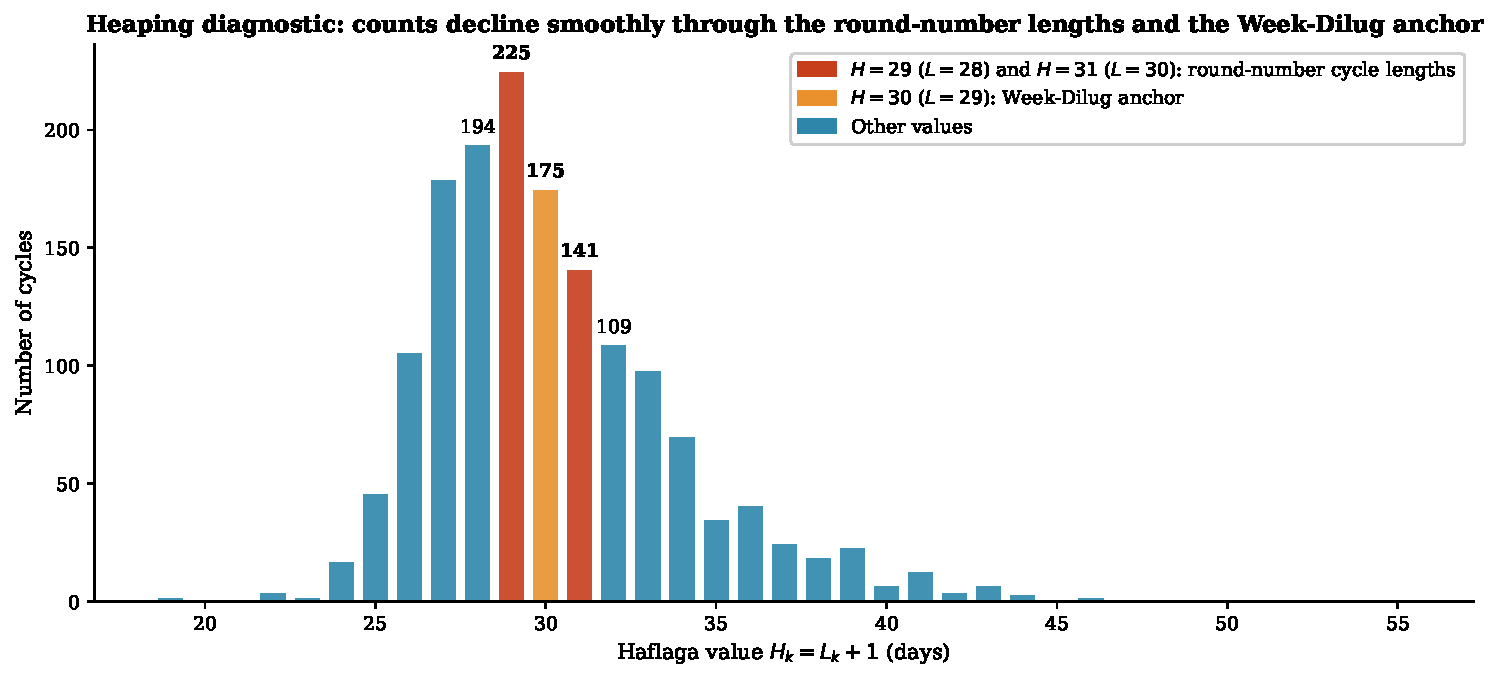
\includegraphics[width=0.88\textwidth]{figA1_heaping_diagnostic}
  \caption{Frequency of each haflaga value $H_k = L_k + 1$ in the analysed sample.
    Red bars: $H = 29$ and $H = 31$, the round-number cycle lengths $L = 28$ and
    $L = 30$ at which digit preference would appear; orange bar: $H = 30$ ($L = 29$),
    the Week-Dilug anchor. Counts decline smoothly through these values
    (225, 175, 141), so the Week-Dilug count does not appear to reflect reporting
    heaping.}
  \label{fig:heaping}
\end{figure}

% ─── 6. Conclusion ────────────────────────────────────────────────────────────
\section{Conclusion}

We applied three exchangeability nulls to the counts of five rule-defined menstrual
patterns in 1,554 cycles from 118 women. Under population-level nulls the count vector is
far in the tail, driven by Haflaga events at 2.3 times their global-null expectation
(26 observed versus 11.3 expected; $z = 4.50$); under a within-woman permutation null
conditional on each woman's own cycle-length values it is not, and all counts lie at or
below their conditional means. Simulation shows type-I error at or below the nominal
level for the marginal and Holm procedures and approximately nominal for the joint test;
under the simulated alternatives the within-woman tests have high power against
exact repetition and against AR(1) dependence of moderate strength (about 50\% at
$\rho = 0.25$, near-certain at $\rho \geq 0.5$); and the conclusions are insensitive to
unequal follow-up. The results are consistent with
between-woman heterogeneity in regularity generating the global excess and provide no
evidence that within-woman ordering adds rule-defined events; they do not establish the
absence of serial dependence, and they say nothing about the forecasting value of the
rules, which is the subject of ongoing work. To our knowledge this is the first formal
randomisation-based test of the halachic vesset rules on empirical data. The general
lesson is that for rule-defined counts in clustered longitudinal sequences the choice of
exchangeability null is the analysis, and that a within-subject conditional null should
be reported alongside any pooled one.

% ─── Ethics Statement ─────────────────────────────────────────────────────────
\section*{Ethics Statement}

This study is a secondary analysis of a publicly archived, anonymised dataset
\citep{fehring2012data} collected in the randomised trial of \citet{fehring2013}. The
original data collection was approved by the Institutional Review Board at Marquette
University. No new data were collected, and no individual participant can be identified
from the released dataset. Separate ethics approval for secondary analysis was not
required under the applicable regulations.

\section*{Patient Consent Statement}

No new data were collected and there was no contact with participants. According to the
archive record of the dataset \citep{fehring2012data}, the human-subject data were
anonymised for dissemination and data reuse was agreed to by the participants in the
original consent form.

\section*{Conflict of Interest}

The author declares no conflicts of interest.

\section*{Data Availability Statement}
\label{sec:das}

The source dataset is publicly available from Marquette University e-Publications
\citep{fehring2012data}. All analyses reported in this article are
reproducible from the released filtered dataset and analysis code at
\url{https://github.com/dvirross/VessetVectorTest}: the filtered data file
(\texttt{data/FilteredData.csv}; SHA-256 fingerprint \texttt{508ee88e\ldots691f7811},
given in full in the Supporting Information and the repository README so that readers can
verify file integrity), the pattern-counting code with an equivalence test between two
implementations, the null-model generators, the simulation validation, the
post-processing script that produces every reported number, the notebook and the
standalone Figure~\ref{fig:consort} script that together produce all figures, and the
cached Monte Carlo replicates ($B = 50{,}000$ per null) that allow
all results to be reproduced without re-simulation.

The preprocessing step is also reproducible. The script
\texttt{scripts/filter\_raw.py} derives the filtered file from the archived source file
(1,665 cycles, 159 women) by removing three women with duplicated cycle records, women
with fewer than 5 recorded cycles, and one duplicated copy of one woman's cycles, and
verifies that its output is identical to the released filtered file; no cycle-length
criterion is applied, all archived lengths already lying between 18 and 54 days. The
copy of the archived source file used by the author (\texttt{data/RawData.csv}) and the
original filtering notebook are included in the code release; the archive itself is
available from the Marquette repository cited above. Women retained
in the filtered file have between 5 and 45 consecutive recorded cycles, and every
retained woman's cycle numbering is contiguous.

% ─── References ───────────────────────────────────────────────────────────────
\bibliographystyle{plainnat}
\bibliography{references}

\end{document}
